\chapter{Comparison of performances} 

\section{Configuration (10 trees)}
\begin{tabular}[b]{|c|c|c|}\hline
      Field & Forest Encoders & SAE \\ \hline
      Features encoded & 10 & 7 \\ \hline
      Random seed & 0 & 0 \\ \hline
\end{tabular}
\subsection*{Apple Overall results}
\begin{tabular}[b]{|c|c|c|}\hline
      Field & Forest Encoders & SAE \\ \hline
      Total Time(9 years) & 1806.40 & 1991.65 \\ \hline
      Features encoded & 10 & 7 \\ \hline
      Encoding Time & 0.93 & 38.67 \\ \hline
      Total Profitability & -26.24\% & -71.65\% \\ \hline
      Average Profitability & -2.91\% & -7.96\% \\ \hline
\end{tabular}
\newpage
\subsection*{Apple Yearly results}
\begin{figure}[!htb]
    \centering
    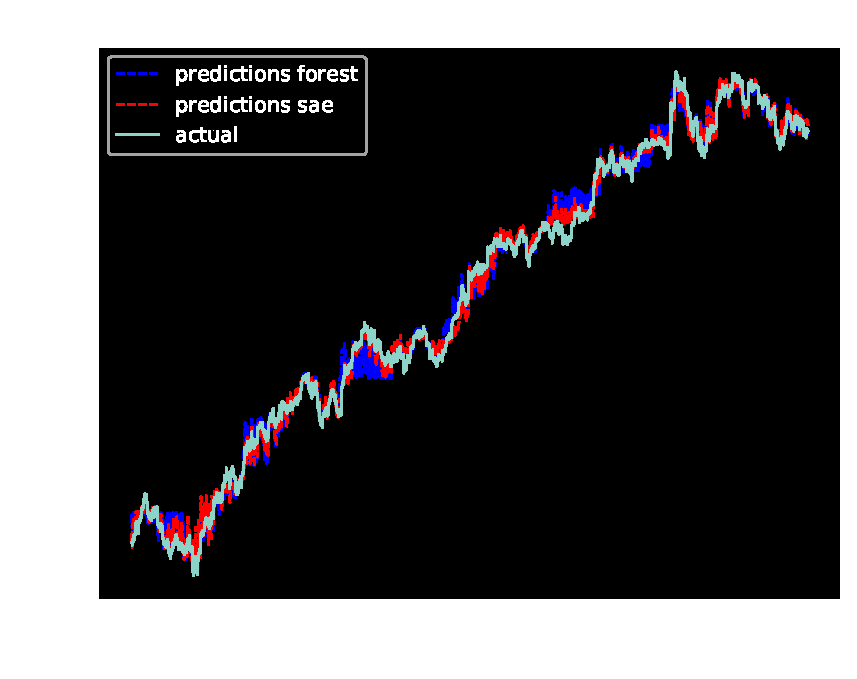
\includegraphics[scale=1]{Appendix3/Figs/rn0f10/APPL_randomSeed_0_forest_no_10_YEAR_2009.pdf}
    \qquad
    \begin{tabular}[b]{|c|c|c|}\hline
      Field & Forest Encoders & SAE \\ \hline
      Data & Apple 2009 & Apple 2009 \\ \hline
      Profitability & -56.46\% & -44.56\% \\ \hline
    \end{tabular}
    \captionlistentry[table]{Results Apple 2009}
    \captionsetup{labelformat=andtable}
    \caption{Comparison of SAE and Forest performances on Apple 2009 data}
\end{figure}
\newpage
\begin{figure}[!htb]
    \centering
    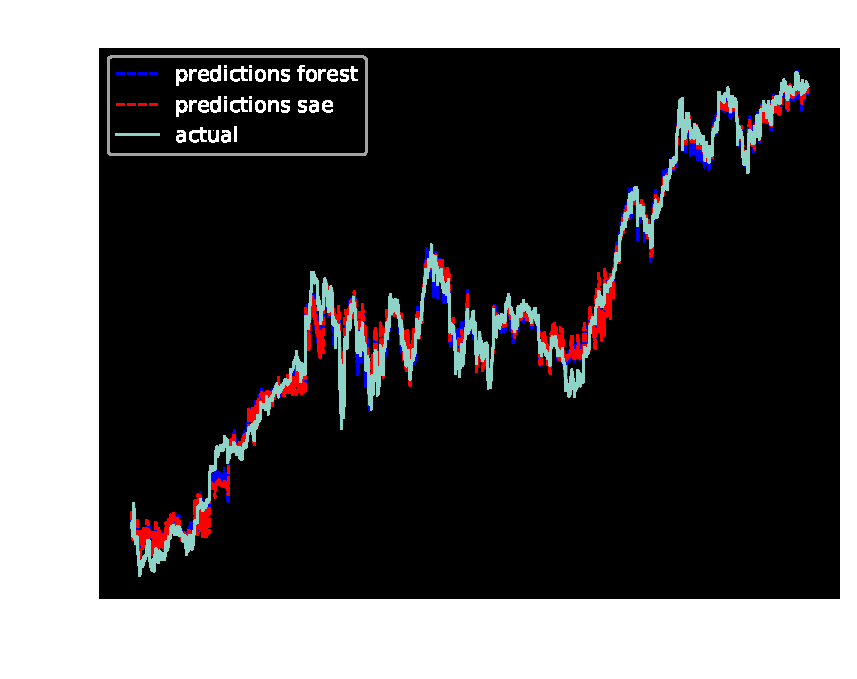
\includegraphics[scale=1]{Appendix3/Figs/rn0f10/APPL_randomSeed_0_forest_no_10_YEAR_2010.pdf}
    \qquad
    \begin{tabular}[b]{|c|c|c|}\hline
      Field & Forest Encoders & SAE \\ \hline
      Data & Apple 2010 & Apple 2010 \\ \hline
      Profitability & -27.36\% & -5.03\% \\ \hline
    \end{tabular}
    \captionlistentry[table]{Results Apple 2010}
    \captionsetup{labelformat=andtable}
    \caption{Comparison of SAE and Forest performances on Apple 2010 data}
\end{figure}
\newpage
\begin{figure}[!htb]
    \centering
    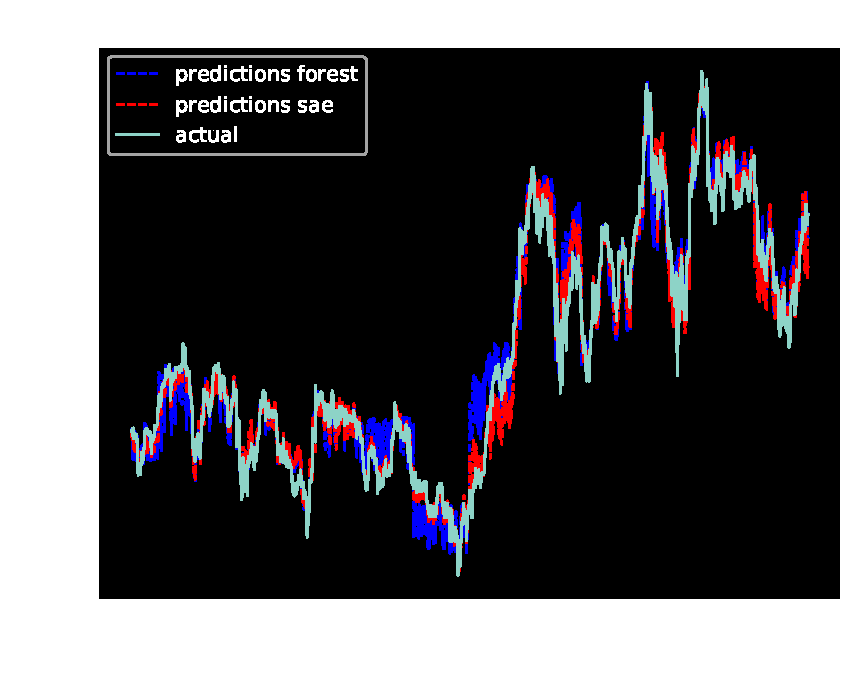
\includegraphics[scale=1]{Appendix3/Figs/rn0f10/APPL_randomSeed_0_forest_no_10_YEAR_2011.pdf}
    \qquad
    \begin{tabular}[b]{|c|c|c|}\hline
      Field & Forest Encoders & SAE \\ \hline
      Data & Apple 2011 & Apple 2011 \\ \hline
      Profitability & 31.60\% & 2.04\% \\ \hline
    \end{tabular}
    \captionlistentry[table]{Results Apple 2011}
    \captionsetup{labelformat=andtable}
    \caption{Comparison of SAE and Forest performances on Apple 2011 data}
\end{figure}
\newcommand{}{}
\begin{figure}[!htb]
    \centering
    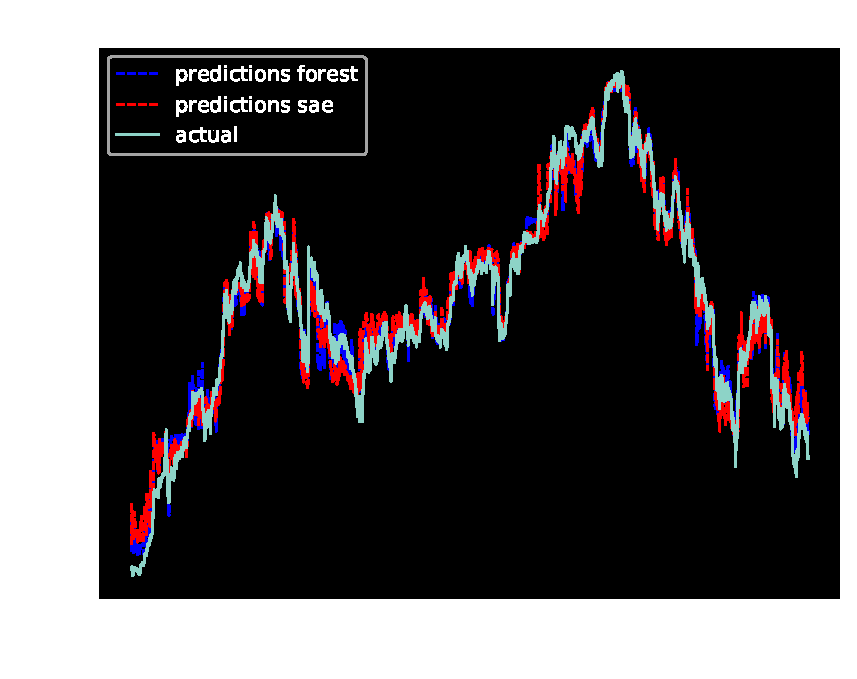
\includegraphics[scale=1]{Appendix3/Figs/rn0f10/APPL_randomSeed_0_forest_no_10_YEAR_2012.pdf}
    \qquad
    \begin{tabular}[b]{|c|c|c|}\hline
      Field & Forest Encoders & SAE \\ \hline
      Data & Apple 2012 & Apple 2012 \\ \hline
      Profitability & 19.27\% & -22.61\% \\ \hline
    \end{tabular}
    \captionlistentry[table]{Results Apple 2012}
    \captionsetup{labelformat=andtable}
    \caption{Comparison of SAE and Forest performances on Apple 2012 data}
\end{figure}
\newpage
\begin{figure}[!htb]
    \centering
    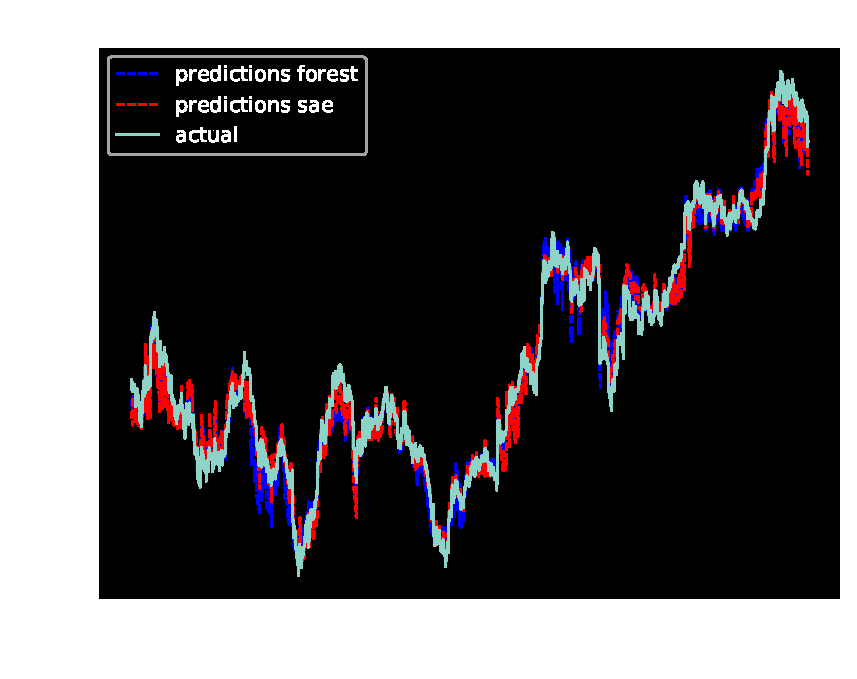
\includegraphics[scale=1]{Appendix3/Figs/rn0f10/APPL_randomSeed_0_forest_no_10_YEAR_2013.pdf}
    \qquad
    \begin{tabular}[b]{|c|c|c|}\hline
      Field & Forest Encoders & SAE \\ \hline
      Data & Apple 2013 & Apple 2013 \\ \hline
      Profitability & -17.30\% & -52.45\% \\ \hline
    \end{tabular}
    \captionlistentry[table]{Results Apple 2013}
    \captionsetup{labelformat=andtable}
    \caption{Comparison of SAE and Forest performances on Apple 2013 data}
\end{figure}
\newpage

\begin{figure}[!htb]
    \centering
    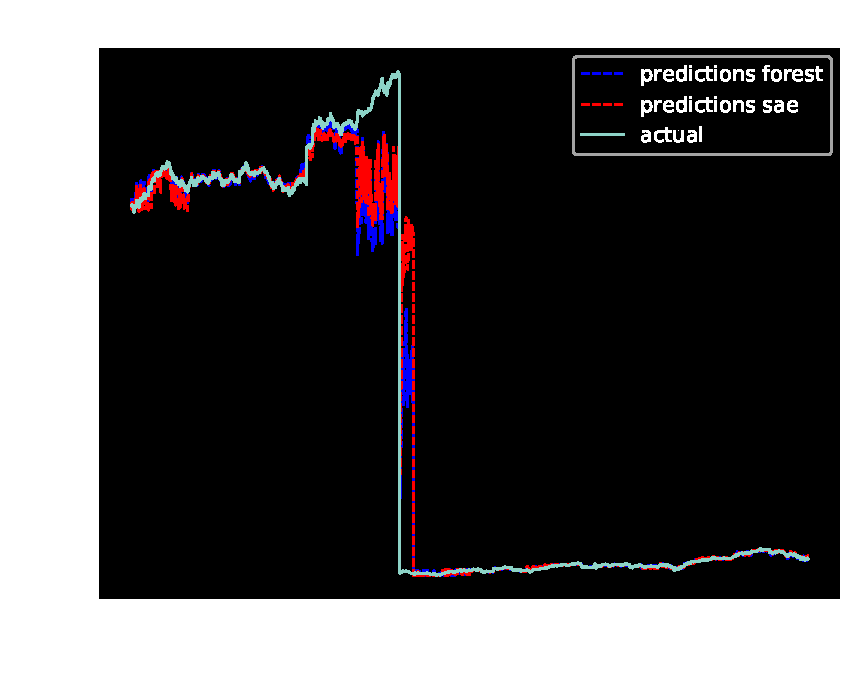
\includegraphics[scale=1]{Appendix3/Figs/rn0f10/APPL_randomSeed_0_forest_no_10_YEAR_2014.pdf}
    \qquad
    \begin{tabular}[b]{|c|c|c|}\hline
      Field & Forest Encoders & SAE \\ \hline
      Data & Apple 2014 & Apple 2014 \\ \hline
      Profitability & 80.13\% & 58.81\% \\ \hline
    \end{tabular}
    \captionlistentry[table]{Results Apple 2014}
    \captionsetup{labelformat=andtable}
    \caption{Comparison of SAE and Forest performances on Apple 2014 data}
\end{figure}
\newpage

\begin{figure}[!htb]
    \centering
    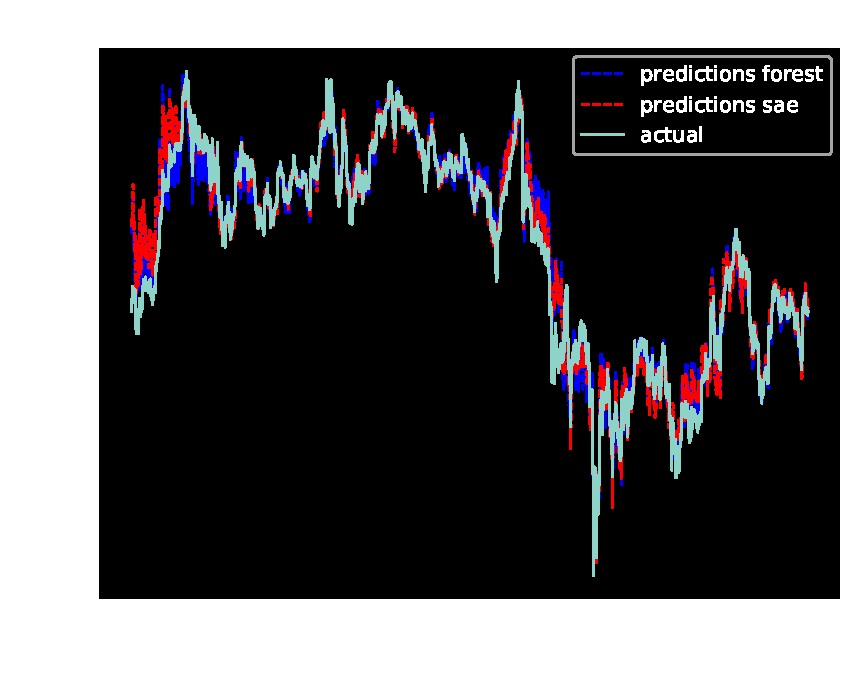
\includegraphics[scale=1]{Appendix3/Figs/rn0f10/APPL_randomSeed_0_forest_no_10_YEAR_2015.pdf}
    \qquad
    \begin{tabular}[b]{|c|c|c|}\hline
      Field & Forest Encoders & SAE \\ \hline
      Data & Apple 2015 & Apple 2015 \\ \hline
      Profitability & -24.11\% & 16.23\% \\ \hline
    \end{tabular}
    \captionlistentry[table]{Results Apple 2015}
    \captionsetup{labelformat=andtable}
    \caption{Comparison of SAE and Forest performances on Apple 2015 data}
\end{figure}
\newpage

\begin{figure}[!htb]
    \centering
    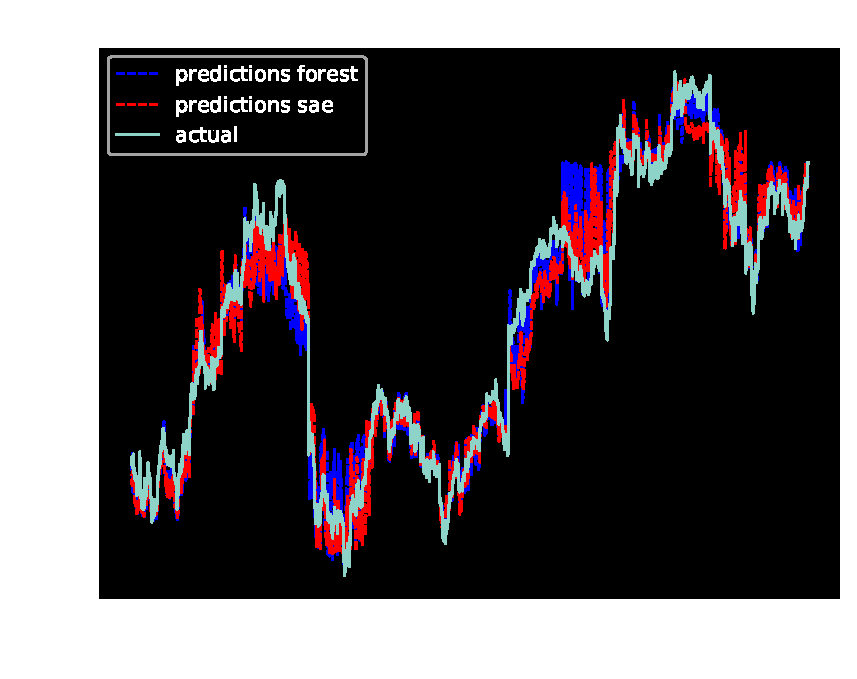
\includegraphics[scale=1]{Appendix3/Figs/rn0f10/APPL_randomSeed_0_forest_no_10_YEAR_2016.pdf}
    \qquad
    \begin{tabular}[b]{|c|c|c|}\hline
      Field & Forest Encoders & SAE \\ \hline
      Data & Apple 2016 & Apple 2016 \\ \hline
      Profitability & -5.14\% & -22.58\% \\ \hline
    \end{tabular}
    \captionlistentry[table]{Results Apple 2016}
    \captionsetup{labelformat=andtable}
    \caption{Comparison of SAE and Forest performances on Apple 2016 data}
\end{figure}
\newpage

\begin{figure}[!htb]
    \centering
    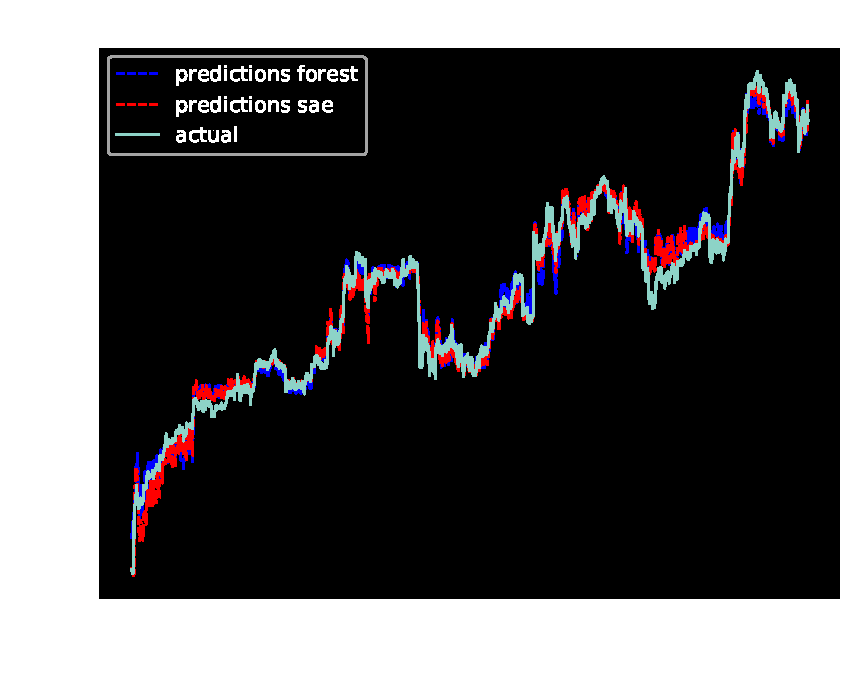
\includegraphics[scale=1]{Appendix3/Figs/rn0f10/APPL_randomSeed_0_forest_no_10_YEAR_2017.pdf}
    \qquad
    \begin{tabular}[b]{|c|c|c|}\hline
      Field & Forest Encoders & SAE \\ \hline
      Data & Apple 2017 & Apple 2017 \\ \hline
      Profitability & -26.86\% & -1.48\% \\ \hline
    \end{tabular}
    \captionlistentry[table]{Results Apple 2017}
    \captionsetup{labelformat=andtable}
    \caption{Comparison of SAE and Forest performances on Apple 2017 data}
\end{figure}
\newpage

%%%%%%%%%%%%%%%%%%%
% RN 5 f 5
%%%%%%%%%%%%%%%%%%%
% \section{Configuration (5 trees)}
% \begin{tabular}[!htb]{|c|c|c|}\hline
%       Field & Forest Encoders & SAE \\ \hline
%       Random seed & 0 & 0 \\ \hline
% \end{tabular}

% \subsection*{Apple Overall results}
% \begin{tabular}[!htb]{|c|c|c|}\hline
%       Field & Forest Encoders & SAE \\ \hline
%       Features encoded & 5 & 7 \\ \hline
%       Total Time(9 years) &  1885.62 & 2026.24 \\ \hline
%       Encoding Time & 0.34 & 39.33 \\ \hline
%       Total Profitability & 126.56\% & -71.65\% \\ \hline
%       Average Profitability & 14.06\% & -7.96\% \\ \hline
% \end{tabular}
% \newpage
% \subsection*{Apple Yearly results}
% \begin{figure}[!htb]
%     \centering
%     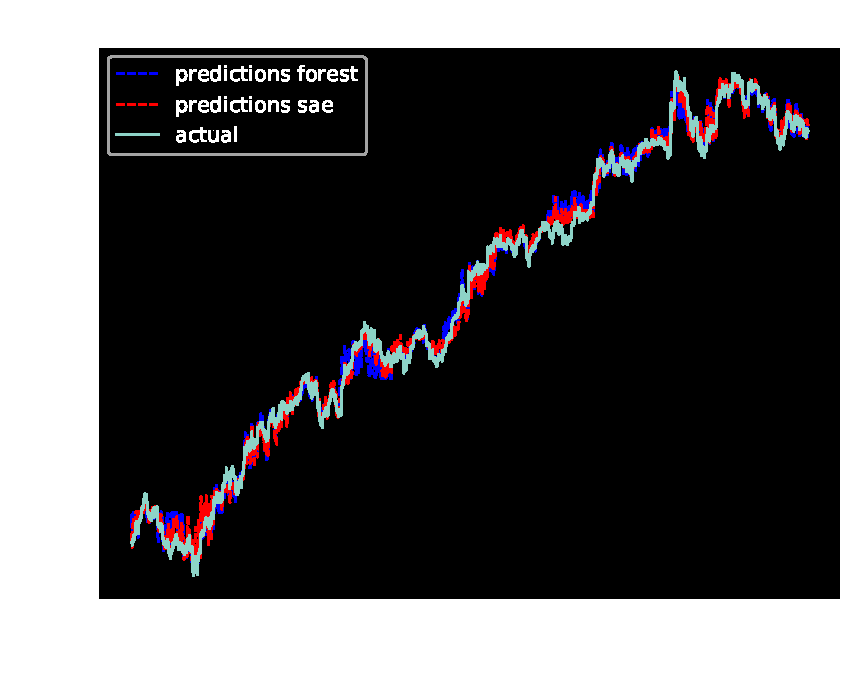
\includegraphics[scale=1]{Appendix3/Figs/rn0f5/APPL_randomSeed_0_forest_no_5_YEAR_2009.png}
%     \qquad
%     \begin{tabular}[b]{|c|c|c|}\hline
%       Field & Forest Encoders & SAE \\ \hline
%       Data & Apple 2009 & Apple 2009 \\ \hline
%       Profitability & -24.31\% & -44.56\% \\ \hline
%     \end{tabular}
%     \captionlistentry[table]{Results Apple 2009}
%     \captionsetup{labelformat=andtable}
%     \caption{Comparison of SAE and Forest performances on Apple 2009 data}
% \end{figure}
% \newpage
% \begin{figure}[!htb]
%     \centering
%     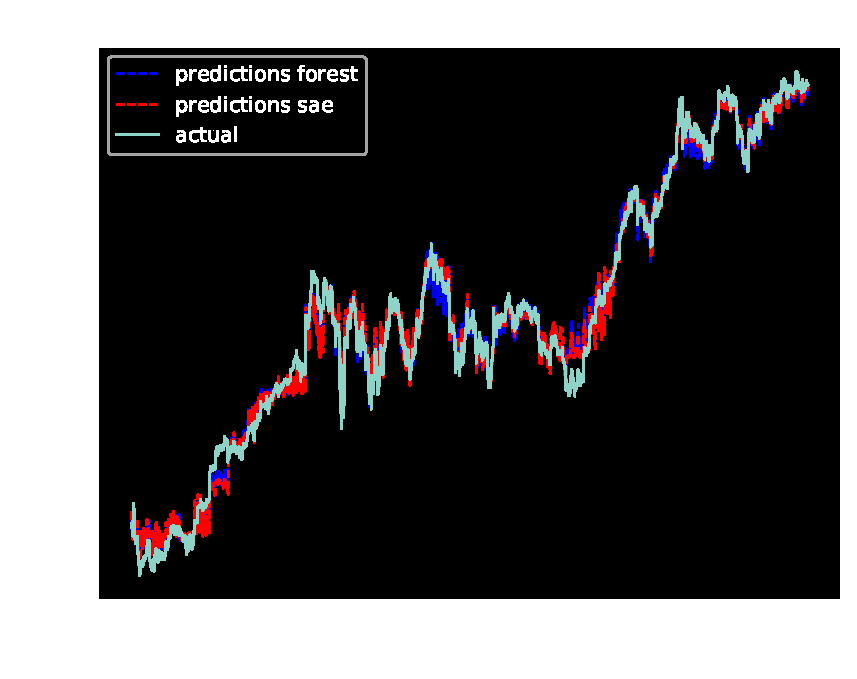
\includegraphics[scale=1]{Appendix3/Figs/rn0f5/APPL_randomSeed_0_forest_no_5_YEAR_2010.png}
%     \qquad
%     \begin{tabular}[b]{|c|c|c|}\hline
%       Field & Forest Encoders & SAE \\ \hline
%       Data & Apple 2010 & Apple 2010 \\ \hline
%       Profitability & 5.40\% & -5.03\% \\ \hline
%     \end{tabular}
%     \captionlistentry[table]{Results Apple 2010}
%     \captionsetup{labelformat=andtable}
%     \caption{Comparison of SAE and Forest performances on Apple 2010 data}
% \end{figure}
% \newpage
% \begin{figure}[!htb]
%     \centering
%     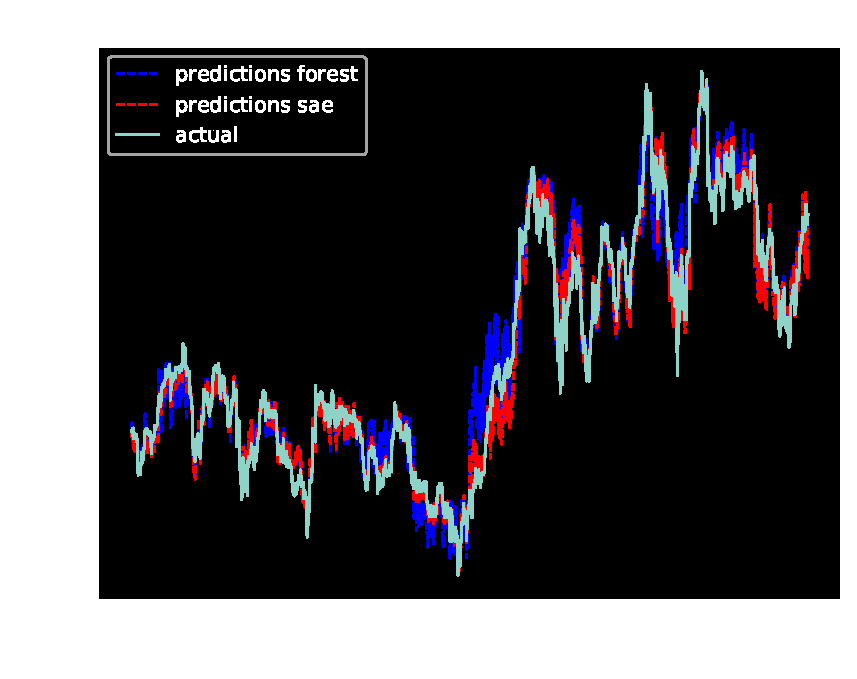
\includegraphics[scale=1]{Appendix3/Figs/rn0f5/APPL_randomSeed_0_forest_no_5_YEAR_2011.png}
%     \qquad
%     \begin{tabular}[b]{|c|c|c|}\hline
%       Field & Forest Encoders & SAE \\ \hline
%       Data & Apple 2011 & Apple 2011 \\ \hline
%       Profitability & 15.70\% & 2.04\% \\ \hline
%     \end{tabular}
%     \captionlistentry[table]{Results Apple 2011}
%     \captionsetup{labelformat=andtable}
%     \caption{Comparison of SAE and Forest performances on Apple 2011 data}
% \end{figure}
% \newpage
% \begin{figure}[!htb]
%     \centering
%     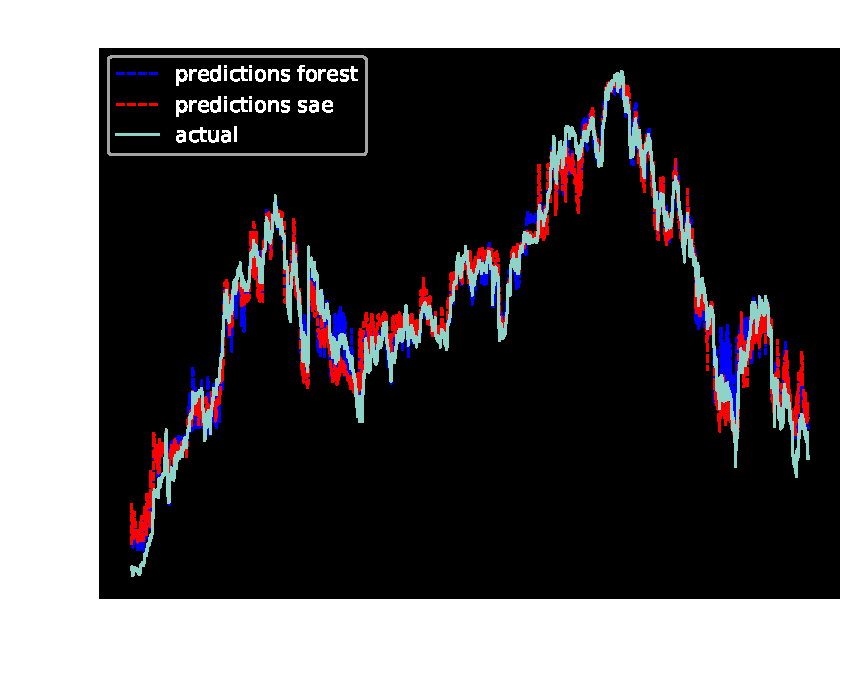
\includegraphics[scale=1]{Appendix3/Figs/rn0f5/APPL_randomSeed_0_forest_no_5_YEAR_2012.png}
%     \qquad
%     \begin{tabular}[b]{|c|c|c|}\hline
%       Field & Forest Encoders & SAE \\ \hline
%       Data & Apple 2012 & Apple 2012 \\ \hline
%       Profitability & 34.61\% &-22.61\% \\ \hline
%     \end{tabular}
%     \captionlistentry[table]{Results Apple 2012}
%     \captionsetup{labelformat=andtable}
%     \caption{Comparison of SAE and Forest performances on Apple 2012 data}
% \end{figure}
% \newpage
% \begin{figure}[!htb]
%     \centering
%     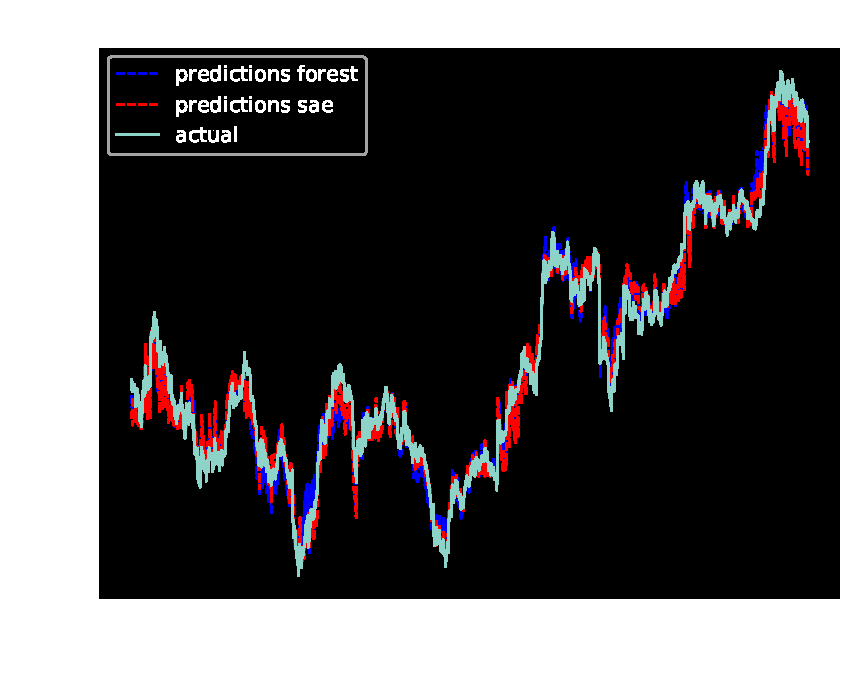
\includegraphics[scale=1]{Appendix3/Figs/rn0f5/APPL_randomSeed_0_forest_no_5_YEAR_2013.png}
%     \qquad
%     \begin{tabular}[b]{|c|c|c|}\hline
%       Field & Forest Encoders & SAE \\ \hline
%       Data & Apple 2013 & Apple 2013 \\ \hline
%       Profitability & -24.64\% &-52.45\% \\ \hline
%     \end{tabular}
%     \captionlistentry[table]{Results Apple 2013}
%     \captionsetup{labelformat=andtable}
%     \caption{Comparison of SAE and Forest performances on Apple 2013 data}
% \end{figure}
% \newpage
% \begin{figure}[!htb]
%     \centering
%     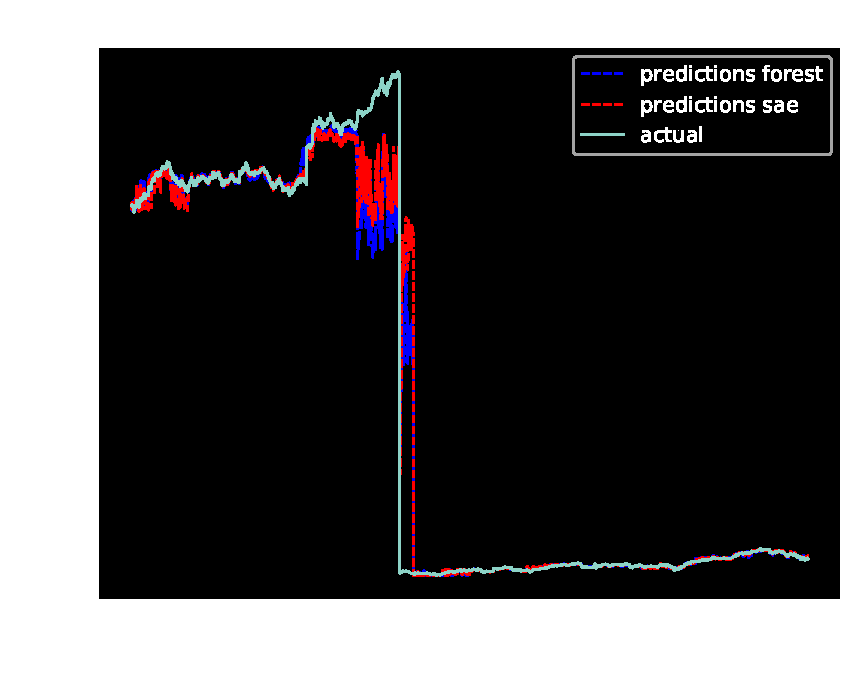
\includegraphics[scale=1]{Appendix3/Figs/rn0f5/APPL_randomSeed_0_forest_no_5_YEAR_2014.png}
%     \qquad
%     \begin{tabular}[b]{|c|c|c|}\hline
%       Field & Forest Encoders & SAE \\ \hline
%       Data & Apple 2014 & Apple 2014 \\ \hline
%       Profitability & 73.57\% &58.81\% \\ \hline
%     \end{tabular}
%     \captionlistentry[table]{Results Apple 2014}
%     \captionsetup{labelformat=andtable}
%     \caption{Comparison of SAE and Forest performances on Apple 2014 data}
% \end{figure}
% \newpage
% \begin{figure}[!htb]
%     \centering
%     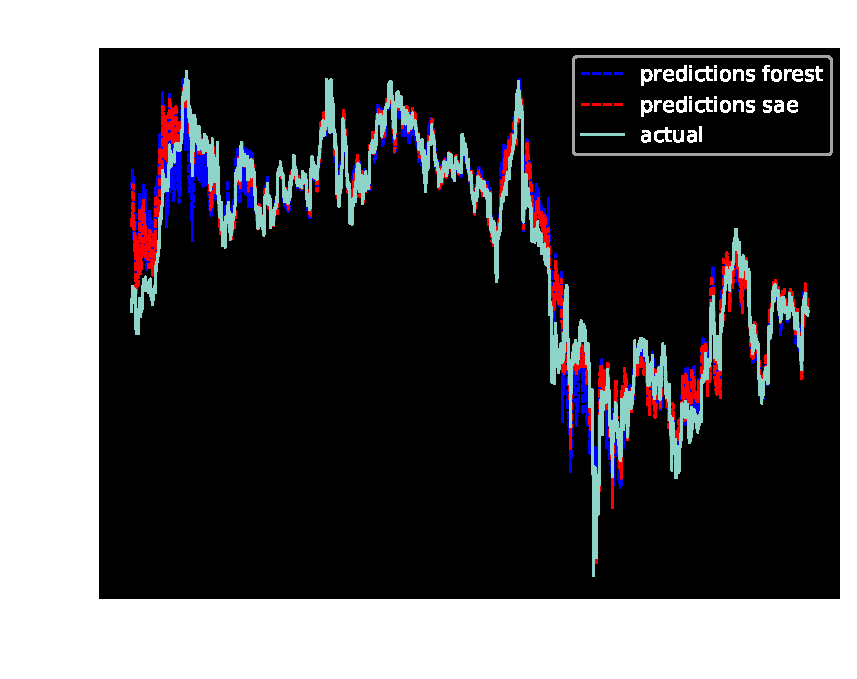
\includegraphics[scale=1]{Appendix3/Figs/rn0f5/APPL_randomSeed_0_forest_no_5_YEAR_2015.png}
%     \qquad
%     \begin{tabular}[b]{|c|c|c|}\hline
%       Field & Forest Encoders & SAE \\ \hline
%       Data & Apple 2015 & Apple 2015 \\ \hline
%       Profitability & 14.75\% &16.23\% \\ \hline
%     \end{tabular}
%     \captionlistentry[table]{Results Apple 2015}
%     \captionsetup{labelformat=andtable}
%     \caption{Comparison of SAE and Forest performances on Apple 2015 data}
% \end{figure}
% \newpage
% \begin{figure}[!htb]
%     \centering
%     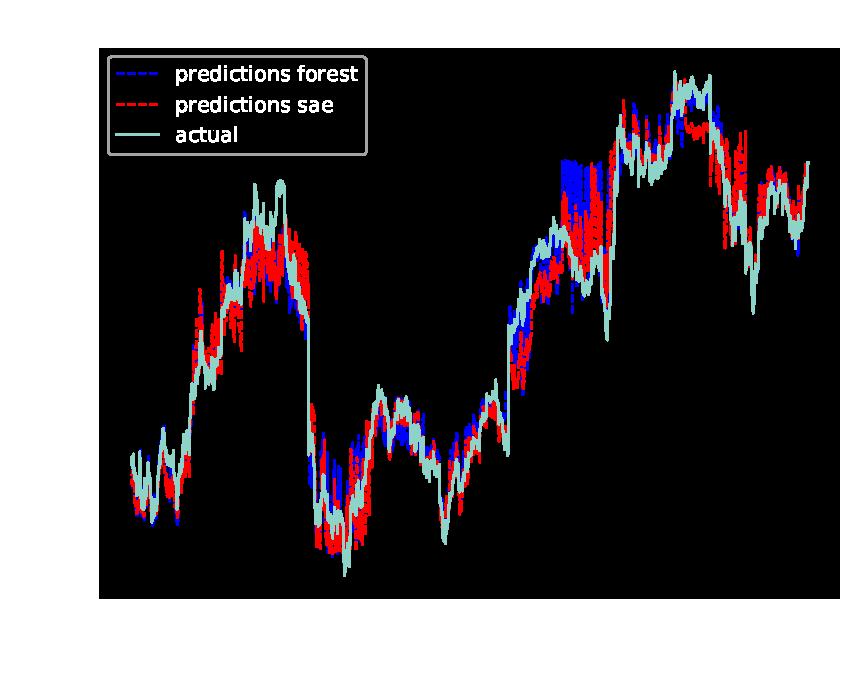
\includegraphics[scale=1]{Appendix3/Figs/rn0f5/APPL_randomSeed_0_forest_no_5_YEAR_2016.png}
%     \qquad
%     \begin{tabular}[b]{|c|c|c|}\hline
%       Field & Forest Encoders & SAE \\ \hline
%       Data & Apple 2016 & Apple 2016 \\ \hline
%       Profitability & 22.90\% &-22.58\% \\ \hline
%     \end{tabular}
%     \captionlistentry[table]{Results Apple 2016}
%     \captionsetup{labelformat=andtable}
%     \caption{Comparison of SAE and Forest performances on Apple 2016 data}
% \end{figure}
% \newpage
% \begin{figure}[!htb]
%     \centering
%     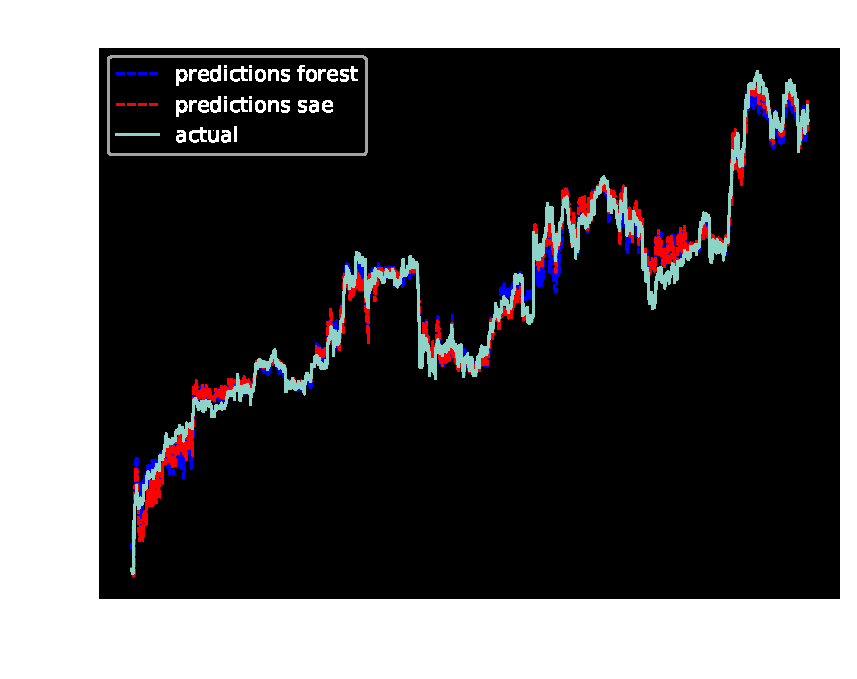
\includegraphics[scale=1]{Appendix3/Figs/rn0f5/APPL_randomSeed_0_forest_no_5_YEAR_2017.png}
%     \qquad
%     \begin{tabular}[b]{|c|c|c|}\hline
%       Field & Forest Encoders & SAE \\ \hline
%       Data & Apple 2017 & Apple 2017 \\ \hline
%       Profitability & 8.56\% &-1.48\% \\ \hline
%     \end{tabular}
%     \captionlistentry[table]{Results Apple 2017}
%     \captionsetup{labelformat=andtable}
%     \caption{Comparison of SAE and Forest performances on Apple 2017 data}
% \end{figure}
% \newpage

% \subsection*{EURO STOXX 50 Overall results}
% \begin{tabular}[!htb]{|c|c|c|}\hline
%       Field & Forest Encoders & SAE \\ \hline
%       Features encoded & 5 & 7 \\ \hline
%       Total Time(6 years) & 3732.03 & 4011.64 \\ \hline
%       Encoding Time & 0.75 & 54.33 \\ \hline
%       Total Profitability & 34.91\% & -67.14\% \\ \hline
%       Average Profitability & 3.87\% & -7.46\% \\ \hline
% \end{tabular}
% \newpage
% \subsection*{EURO STOXX 50 Yearly results}
% \begin{figure}[!htb]
%     \centering
%     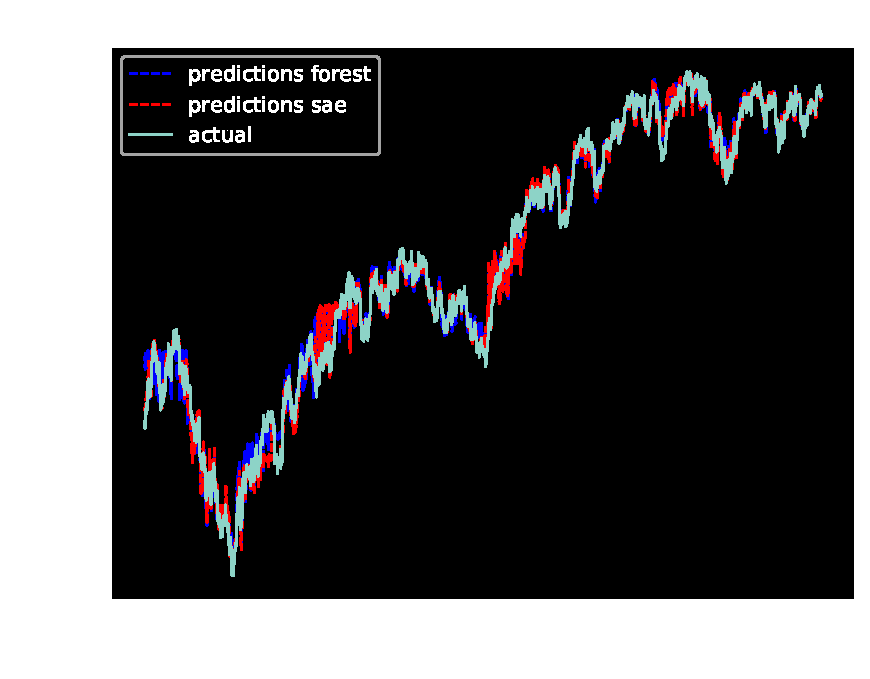
\includegraphics[scale=1]{Appendix3/Figs/rn0f5/eure_randomSeed_0_forest_no_5_YEAR_2009.png}
%     \qquad
%     \begin{tabular}[b]{|c|c|c|}\hline
%       Field & Forest Encoders & SAE \\ \hline
%       Data & EURO STOXX 50 2009 & EURO STOXX 50 2009\\ \hline
%       Profitability & 35.06\% & 33.30\% \\ \hline
%     \end{tabular}
%     \captionlistentry[table]{Results EURO STOXX 50 2009}
%     \captionsetup{labelformat=andtable}
%     \caption{Comparison of SAE and Forest performances on EURO STOXX 50 2009 data}
% \end{figure}
% \newpage
% \begin{figure}[!htb]
%     \centering
%     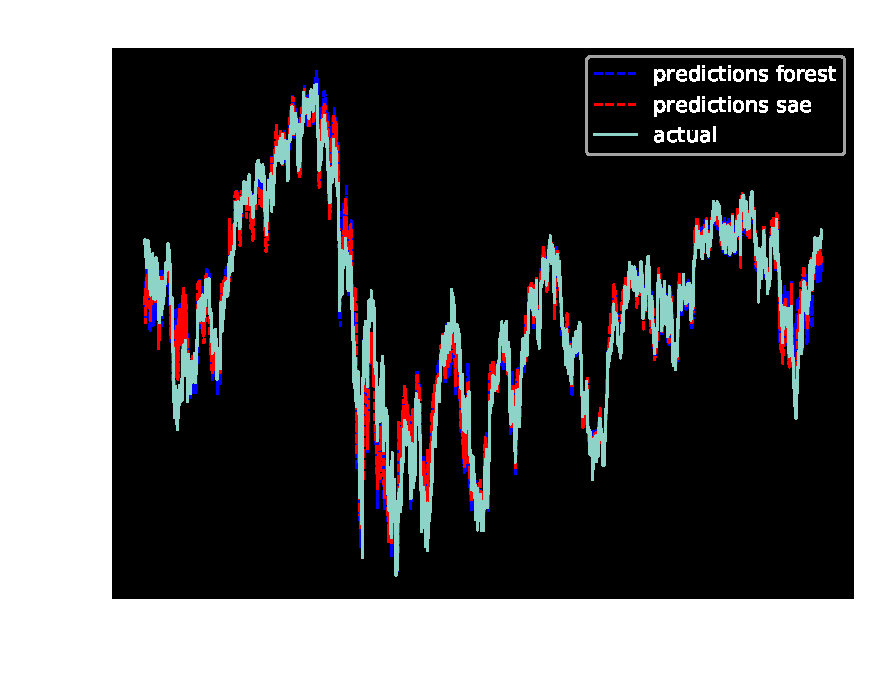
\includegraphics[scale=1]{Appendix3/Figs/rn0f5/eure_randomSeed_0_forest_no_5_YEAR_2010.png}
%     \qquad
%     \begin{tabular}[b]{|c|c|c|}\hline
%       Field & Forest Encoders & SAE \\ \hline
%       Data & EURO STOXX 50 2010 & EURO STOXX 50 2010\\ \hline
%       Profitability & 4.71\% & -8.13\% \\ \hline
%     \end{tabular}
%     \captionlistentry[table]{Results EURO STOXX 50 2010}
%     \captionsetup{labelformat=andtable}
%     \caption{Comparison of SAE and Forest performances on EURO STOXX 50 2010 data}
% \end{figure}

% \newpage
% \begin{figure}[!htb]
%     \centering
%     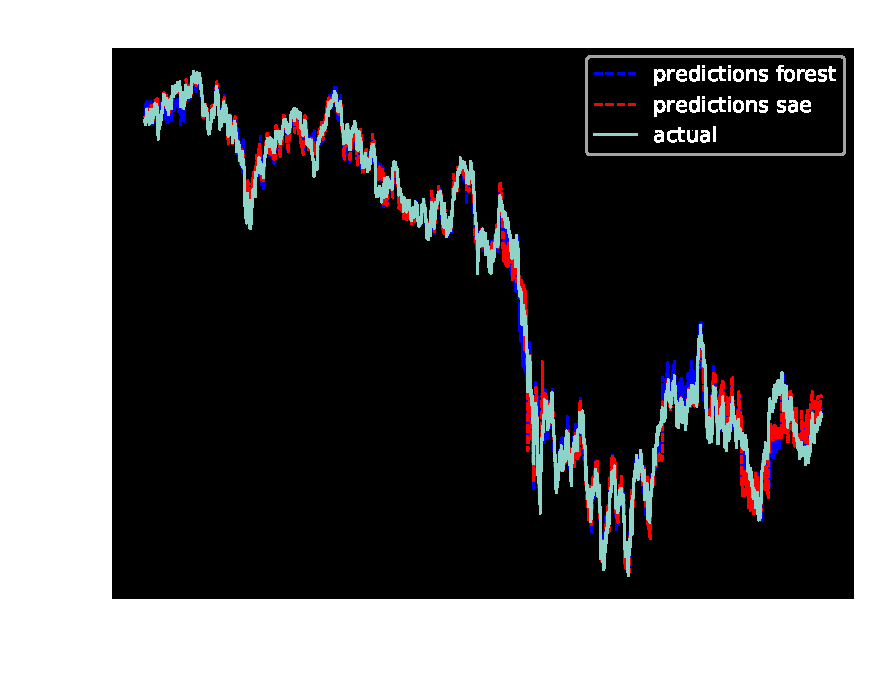
\includegraphics[scale=1]{Appendix3/Figs/rn0f5/eure_randomSeed_0_forest_no_5_YEAR_2011.png}
%     \qquad
%     \begin{tabular}[b]{|c|c|c|}\hline
%       Field & Forest Encoders & SAE \\ \hline
%       Data & EURO STOXX 50 2011 & EURO STOXX 50 2011\\ \hline
%       Profitability & 4.63\% & -52.41\% \\ \hline
%     \end{tabular}
%     \captionlistentry[table]{Results EURO STOXX 50 2011}
%     \captionsetup{labelformat=andtable}
%     \caption{Comparison of SAE and Forest performances on EURO STOXX 50 2011 data}
% \end{figure}
% \newpage
% \begin{figure}[!htb]
%     \centering
%     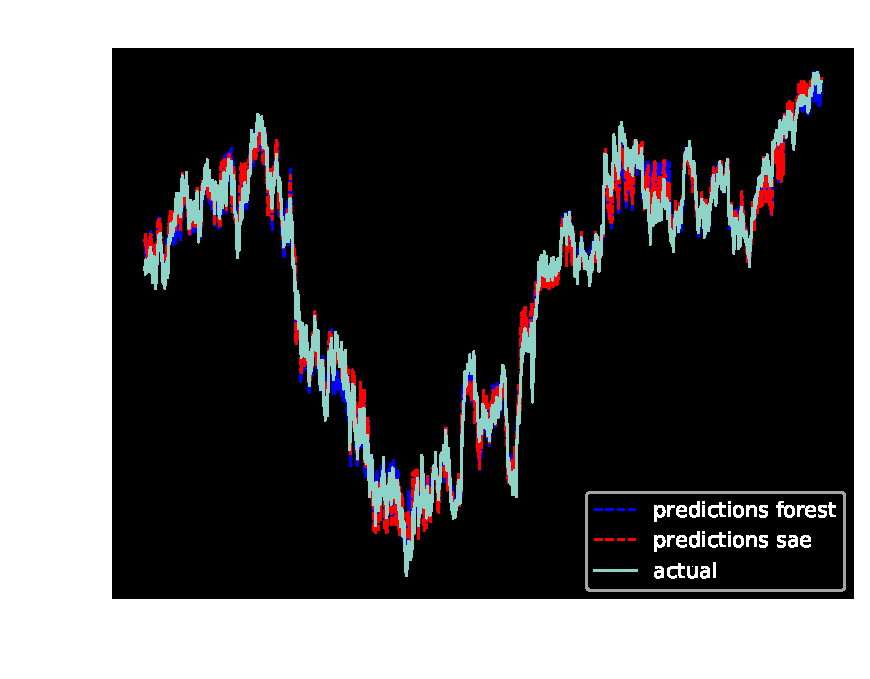
\includegraphics[scale=1]{Appendix3/Figs/rn0f5/eure_randomSeed_0_forest_no_5_YEAR_2012.png}
%     \qquad
%     \begin{tabular}[b]{|c|c|c|}\hline
%       Field & Forest Encoders & SAE \\ \hline
%       Data & EURO STOXX 50 2012 & EURO STOXX 50 2012\\ \hline
%       Profitability & 4.97\% & 0.04\% \\ \hline
%     \end{tabular}
%     \captionlistentry[table]{Results EURO STOXX 50 2012}
%     \captionsetup{labelformat=andtable}
%     \caption{Comparison of SAE and Forest performances on EURO STOXX 50 2012 data}
% \end{figure}
% \newpage
% \begin{figure}[!htb]
%     \centering
%     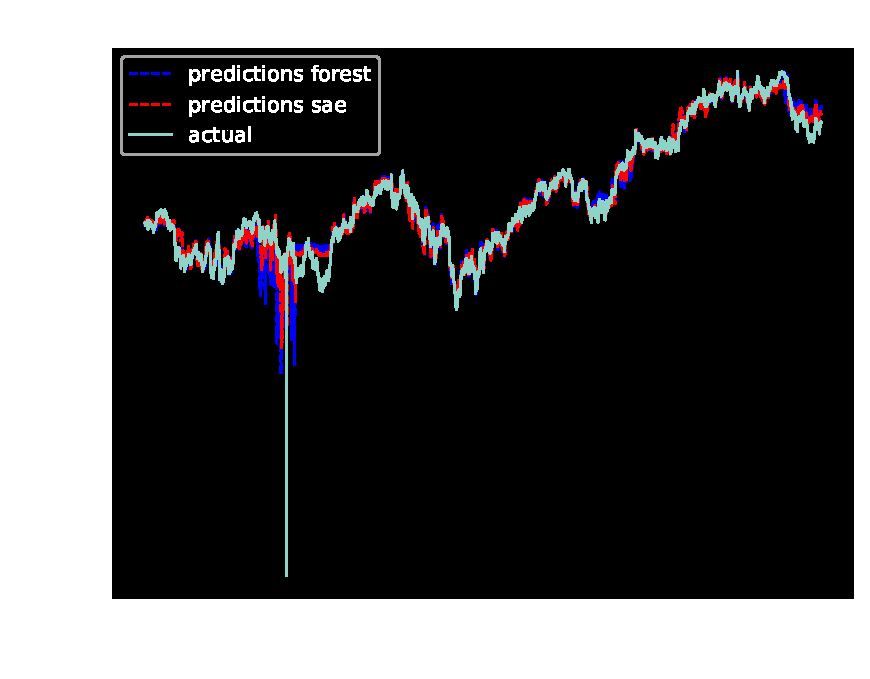
\includegraphics[scale=1]{Appendix3/Figs/rn0f5/eure_randomSeed_0_forest_no_5_YEAR_2013.png}
%     \qquad
%     \begin{tabular}[b]{|c|c|c|}\hline
%       Field & Forest Encoders & SAE \\ \hline
%       Data & EURO STOXX 50 2013 & EURO STOXX 50 2013\\ \hline
%       Profitability & -11.01\% & -14.99\% \\ \hline
%     \end{tabular}
%     \captionlistentry[table]{Results EURO STOXX 50 2013}
%     \captionsetup{labelformat=andtable}
%     \caption{Comparison of SAE and Forest performances on EURO STOXX 50 2013 data}
% \end{figure}
% \newpage
% \begin{figure}[!htb]
%     \centering
%     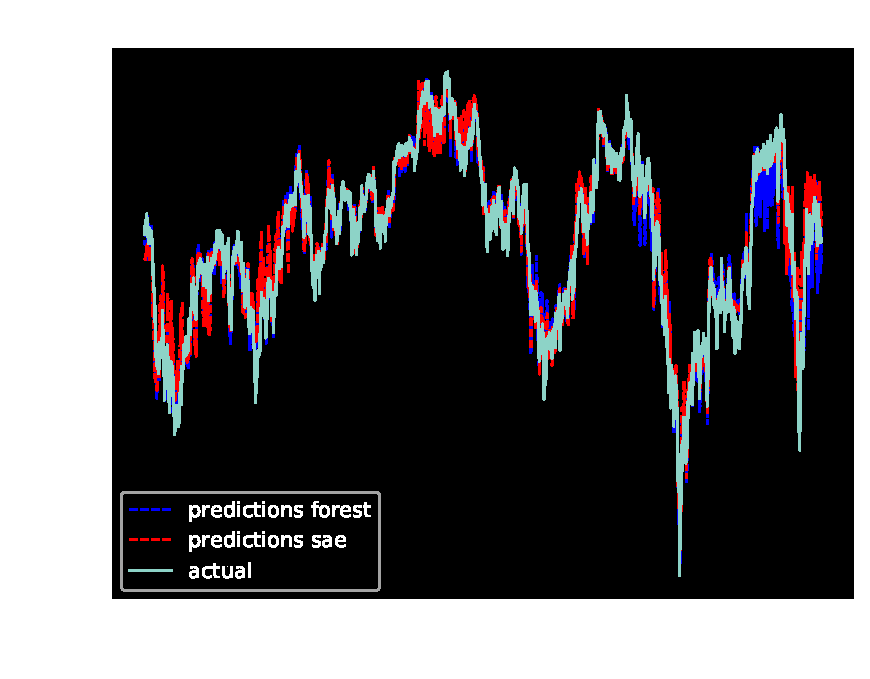
\includegraphics[scale=1]{Appendix3/Figs/rn0f5/eure_randomSeed_0_forest_no_5_YEAR_2014.png}
%     \qquad
%     \begin{tabular}[b]{|c|c|c|}\hline
%       Field & Forest Encoders & SAE \\ \hline
%       Data & EURO STOXX 50 2014 & EURO STOXX 50 2014\\ \hline
%       Profitability & -1.42\% & -1.47\% \\ \hline
%     \end{tabular}
%     \captionlistentry[table]{Results EURO STOXX 50 2014}
%     \captionsetup{labelformat=andtable}
%     \caption{Comparison of SAE and Forest performances on EURO STOXX 50 2014 data}
% \end{figure}
% \newpage
% \begin{figure}[!htb]
%     \centering
%     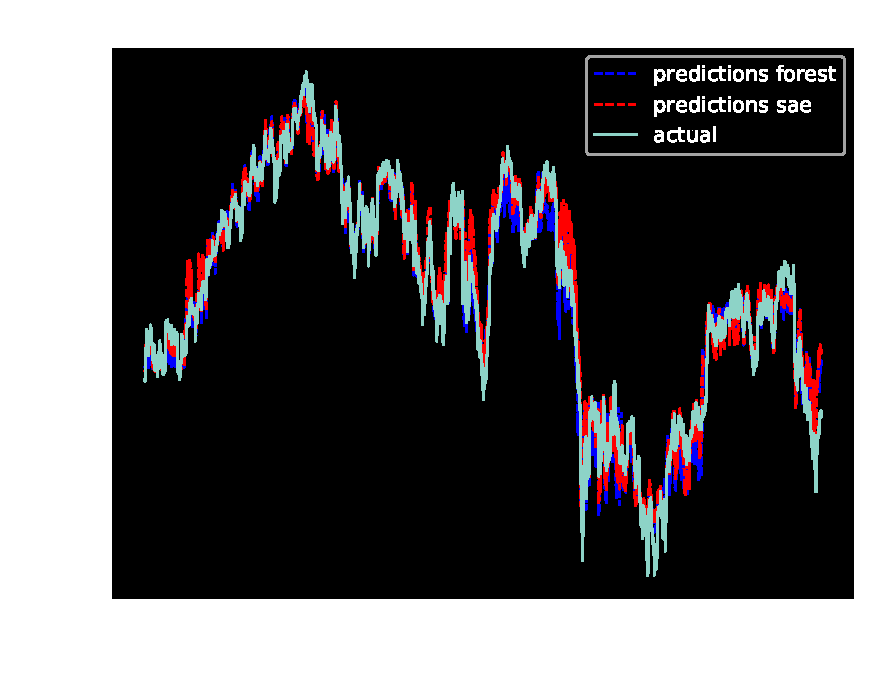
\includegraphics[scale=1]{Appendix3/Figs/rn0f5/eure_randomSeed_0_forest_no_5_YEAR_2015.png}
%     \qquad
%     \begin{tabular}[b]{|c|c|c|}\hline
%       Field & Forest Encoders & SAE \\ \hline
%       Data & EURO STOXX 50 2015 & EURO STOXX 50 2015\\ \hline
%       Profitability & -0.77\% & -11.81\% \\ \hline
%     \end{tabular}
%     \captionlistentry[table]{Results EURO STOXX 50 2015}
%     \captionsetup{labelformat=andtable}
%     \caption{Comparison of SAE and Forest performances on EURO STOXX 50 2015 data}
% \end{figure}
% \newpage
% \begin{figure}[!htb]
%     \centering
%     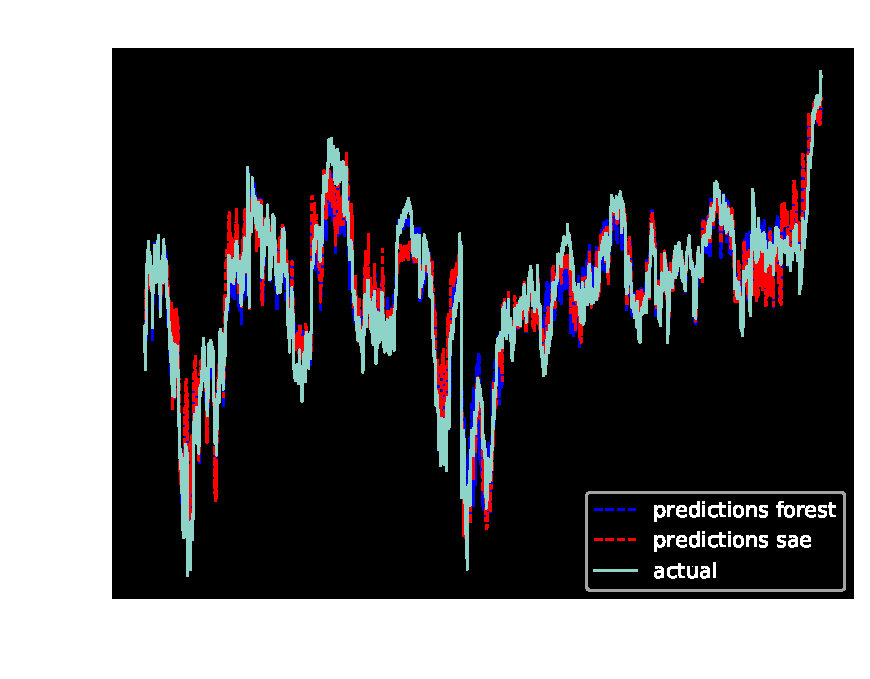
\includegraphics[scale=1]{Appendix3/Figs/rn0f5/eure_randomSeed_0_forest_no_5_YEAR_2016.png}
%     \qquad
%     \begin{tabular}[b]{|c|c|c|}\hline
%       Field & Forest Encoders & SAE \\ \hline
%       Data & EURO STOXX 50 2016 & EURO STOXX 50 2016\\ \hline
%       Profitability & -0.95\% & -1.14\% \\ \hline
%     \end{tabular}
%     \captionlistentry[table]{Results EURO STOXX 50 2016}
%     \captionsetup{labelformat=andtable}
%     \caption{Comparison of SAE and Forest performances on EURO STOXX 50 2016 data}
% \end{figure}
% \newpage
% \begin{figure}[!htb]
%     \centering
%     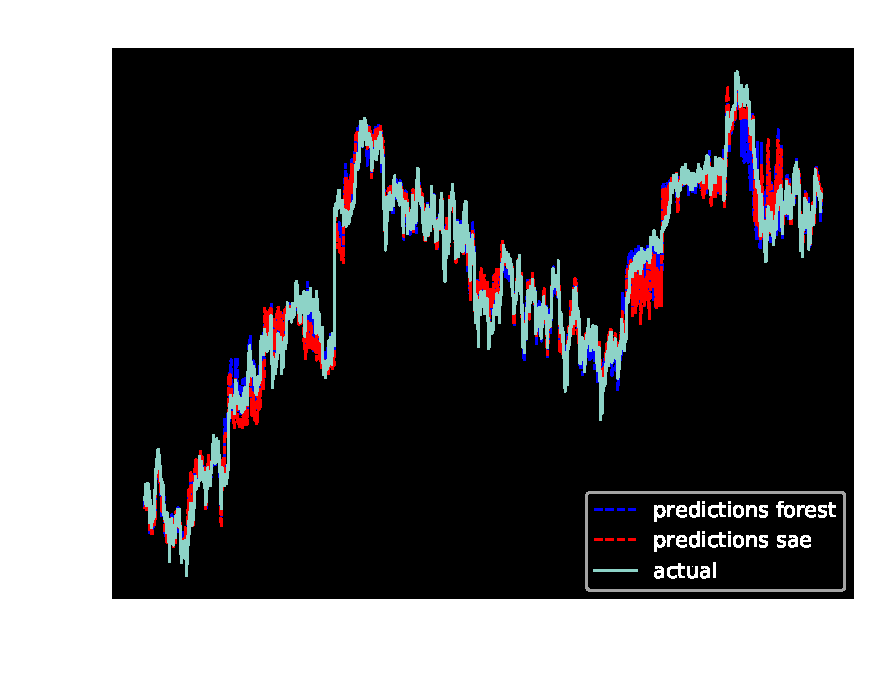
\includegraphics[scale=1]{Appendix3/Figs/rn0f5/eure_randomSeed_0_forest_no_5_YEAR_2017.png}
%     \qquad
%     \begin{tabular}[b]{|c|c|c|}\hline
%       Field & Forest Encoders & SAE \\ \hline
%       Data & EURO STOXX 50 2017 & EURO STOXX 50 2017\\ \hline
%       Profitability & -0.30\% & -10.52\% \\ \hline
%     \end{tabular}
%     \captionlistentry[table]{Results EURO STOXX 50 2017}
%     \captionsetup{labelformat=andtable}
%     \caption{Comparison of SAE and Forest performances on EURO STOXX 50 data 2017}
% \end{figure}

% \newpage
% \subsection*{Netflix Overall results}
% \begin{tabular}[!htb]{|c|c|c|}\hline
%       Field & Forest Encoders & SAE \\ \hline
%       Features encoded & 5 & 6 \\ \hline
%       Total Time(6 years) & 911.62 & 964.32 \\ \hline
%       Encoding Time & 0.34 & 26.74 \\ \hline
%       Total Profitability & 20.74\% & 197.15\% \\ \hline
%       Average Profitability & 2.30\% & 21.90\% \\ \hline
% \end{tabular}
% \newpage
% \subsection*{Netflix Yearly results}
% \begin{figure}[!htb]
%     \centering
%     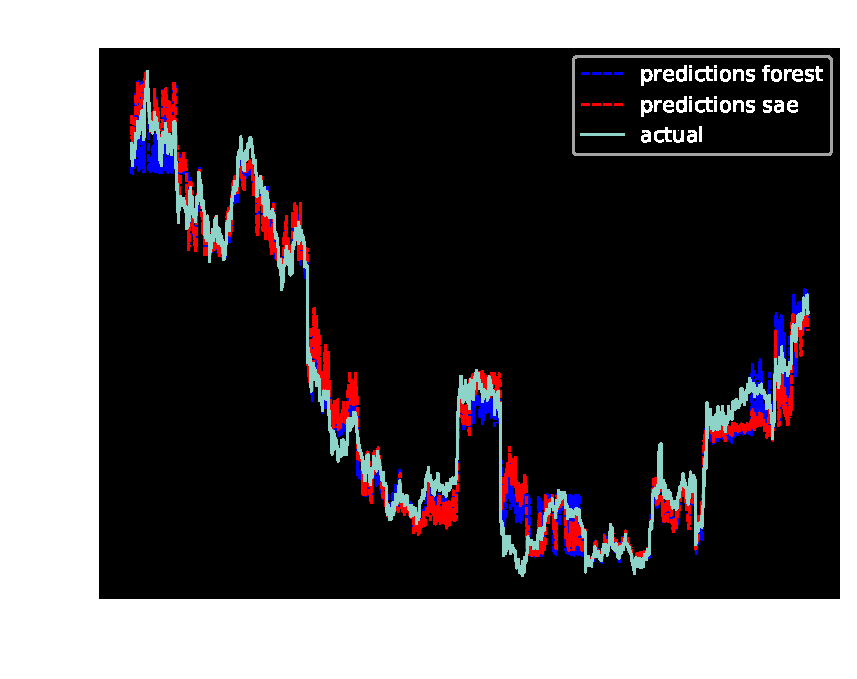
\includegraphics[scale=1]{Appendix3/Figs/rn0f5/NFLX_randomSeed_0_forest_no_5_YEAR_2012.png}
%     \qquad
%     \begin{tabular}[b]{|c|c|c|}\hline
%       Field & Forest Encoders & SAE \\ \hline
%       Data & Netflix 2012 & Netflix 2012 \\ \hline
%       Profitability & 100.69\% & 6.60\% \\ \hline
%     \end{tabular}
%     \captionlistentry[table]{Results Netflix 2012}
%     \captionsetup{labelformat=andtable}
%     \caption{Comparison of SAE and Forest performances on Netflix 2012 data}
% \end{figure}
% \newpage

% \begin{figure}[!htb]
%     \centering
%     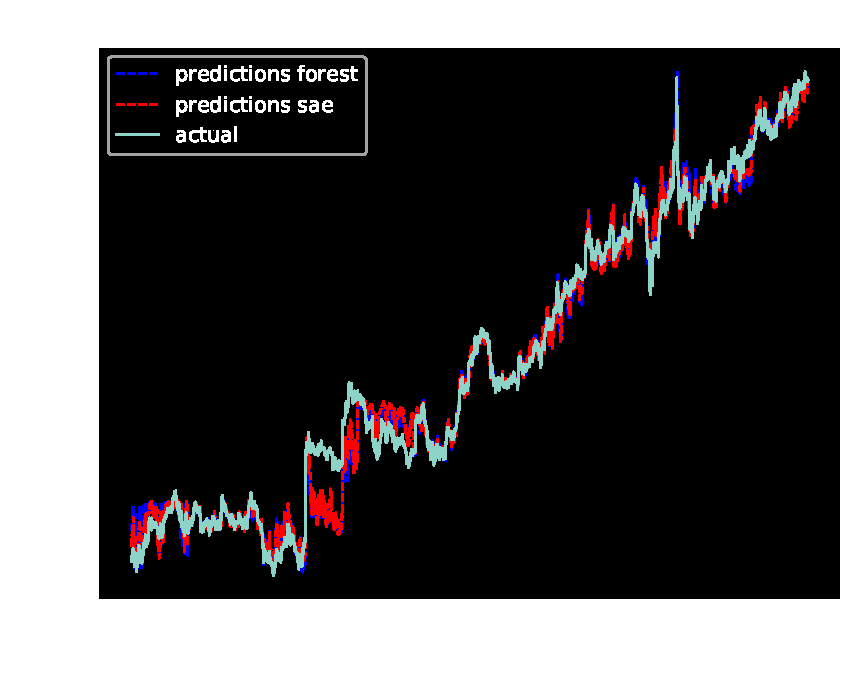
\includegraphics[scale=1]{Appendix3/Figs/rn0f5/NFLX_randomSeed_0_forest_no_5_YEAR_2013.png}
%     \qquad
%     \begin{tabular}[b]{|c|c|c|}\hline
%       Field & Forest Encoders & SAE \\ \hline
%       Data & Netflix 2013 & Netflix 2013 \\ \hline
%       Profitability & 6.07\% & -49.88\% \\ \hline
%     \end{tabular}
%     \captionlistentry[table]{Results Netflix 2013}
%     \captionsetup{labelformat=andtable}
%     \caption{Comparison of SAE and Forest performances on Netflix 2013 data}
% \end{figure}
% \newpage

% \begin{figure}[!htb]
%     \centering
%     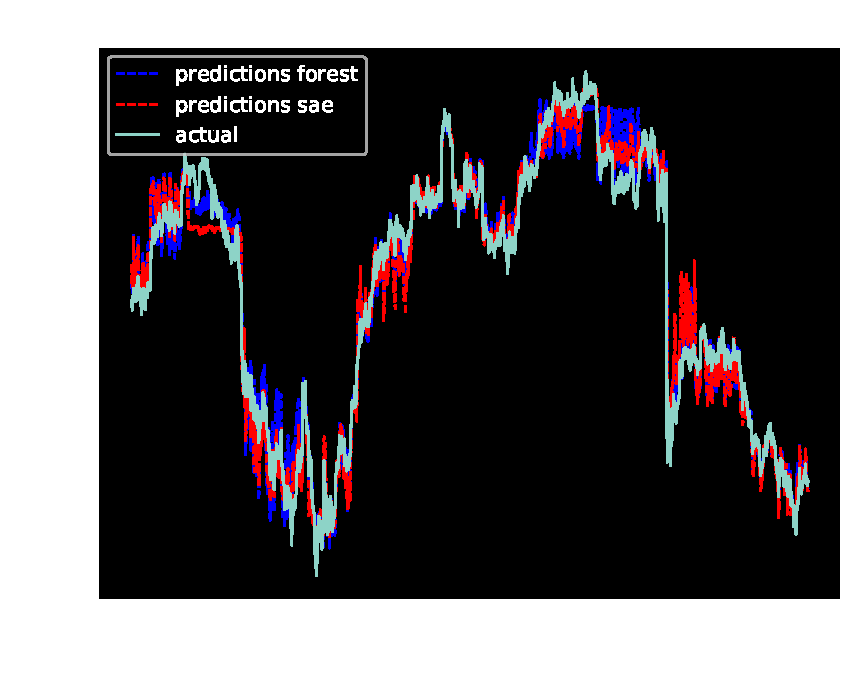
\includegraphics[scale=1]{Appendix3/Figs/rn0f5/NFLX_randomSeed_0_forest_no_5_YEAR_2014.png}
%     \qquad
%     \begin{tabular}[b]{|c|c|c|}\hline
%       Field & Forest Encoders & SAE \\ \hline
%       Data & Netflix 2014 & Netflix 2014 \\ \hline
%       Profitability & 31.25\% & 74.99\% \\ \hline
%     \end{tabular}
%     \captionlistentry[table]{Results Netflix 2014}
%     \captionsetup{labelformat=andtable}
%     \caption{Comparison of SAE and Forest performances on Netflix 2014 data}
% \end{figure}
% \newpage

% \begin{figure}[!htb]
%     \centering
%     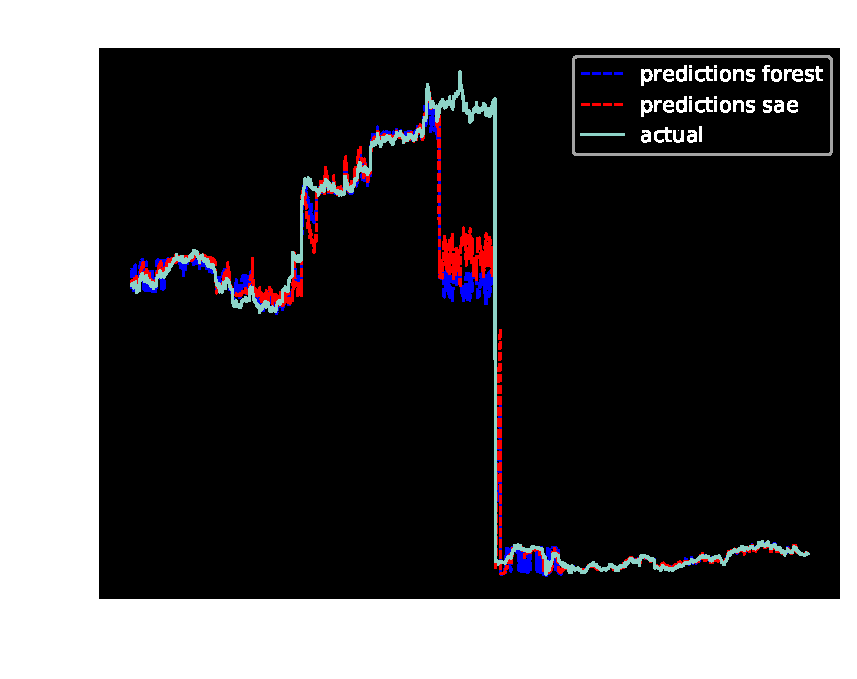
\includegraphics[scale=1]{Appendix3/Figs/rn0f5/NFLX_randomSeed_0_forest_no_5_YEAR_2015.png}
%     \qquad
%     \begin{tabular}[b]{|c|c|c|}\hline
%       Field & Forest Encoders & SAE \\ \hline
%       Data & Netflix 2015 & Netflix 2015 \\ \hline
%       Profitability & -88.68\% & 110.56\% \\ \hline
%     \end{tabular}
%     \captionlistentry[table]{Results Netflix 2016}
%     \captionsetup{labelformat=andtable}
%     \caption{Comparison of SAE and Forest performances on Netflix 2015 data}
% \end{figure}
% \newpage

% \begin{figure}[!htb]
%     \centering
%     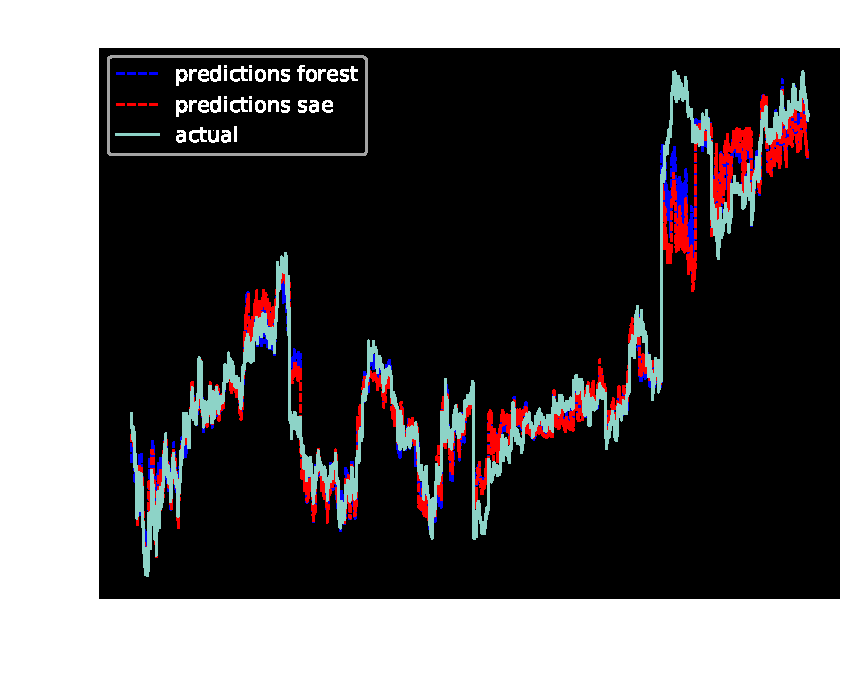
\includegraphics[scale=1]{Appendix3/Figs/rn0f5/NFLX_randomSeed_0_forest_no_5_YEAR_2016.png}
%     \qquad
%     \begin{tabular}[b]{|c|c|c|}\hline
%       Field & Forest Encoders & SAE \\ \hline
%       Data & Netflix 2016 & Netflix 2016 \\ \hline
%       Profitability & -62.12\% &22.41\% \\ \hline
%     \end{tabular}
%     \captionlistentry[table]{Results Netflix 2016}
%     \captionsetup{labelformat=andtable}
%     \caption{Comparison of SAE and Forest performances on Netflix 2016 data}
% \end{figure}
% \newpage

% \begin{figure}[!htb]
%     \centering
%     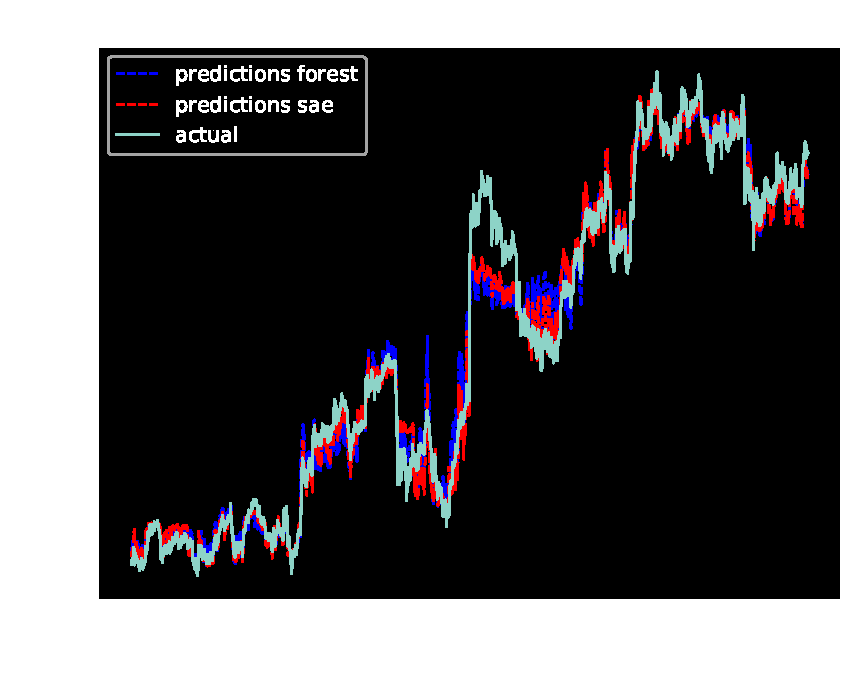
\includegraphics[scale=1]{Appendix3/Figs/rn0f5/NFLX_randomSeed_0_forest_no_5_YEAR_2017.png}
%     \qquad
%     \begin{tabular}[b]{|c|c|c|}\hline
%       Field & Forest Encoders & SAE \\ \hline
%       Data & Netflix 2017 & Netflix 2017 \\ \hline
%       Profitability & 33.52\% &32.45\% \\ \hline
%     \end{tabular}
%     \captionlistentry[table]{Results Netflix 2017}
%     \captionsetup{labelformat=andtable}
%     \caption{Comparison of SAE and Forest performances on Netflix 2017 data}
% \end{figure}

% \newpage
% \subsection*{Nasdaq 100 Overall results}
% \begin{tabular}[!htb]{|c|c|c|}\hline
%       Field & Forest Encoders & SAE \\ \hline
%       Features encoded & 5 & 6 \\ \hline
%       Total Time(8 years) (seconds) & 68434.56 & 54239.25 \\ \hline
%       Encoding Time (seconds) & 2.06 & 136.07 \\ \hline
%       Total Profitability & 157.35\% & 36.44\% \\ \hline
%       Average Profitability & 19.66\% & 4.55\% \\ \hline
% \end{tabular}
% \newpage
% \subsection*{Nasdaq 100 Yearly results}

% \begin{figure}[!htb]
%     \centering
%     \includegraphics[scale=1]{Appendix3/Figs/rn0f5/NQ10_randomSeed_0_forest_no_5_YEAR_2010.png}
%     \qquad
%     \begin{tabular}[b]{|c|c|c|}\hline
%       Field & Forest Encoders & SAE \\ \hline
%       Data & Nasdaq 2010 & Nasdaq 2010 \\ \hline
%       Profitability & 142.05\% &-54.36\% \\ \hline
%     \end{tabular}
%     \captionlistentry[table]{Results Nasdaq 2010}
%     \captionsetup{labelformat=andtable}
%     \caption{Comparison of SAE and Forest performances on Nasdaq 2010 data}
% \end{figure}
% \newpage

% \begin{figure}[!htb]
%     \centering
%     \includegraphics[scale=1]{Appendix3/Figs/rn0f5/NQ10_randomSeed_0_forest_no_5_YEAR_2011.png}
%     \qquad
%     \begin{tabular}[b]{|c|c|c|}\hline
%       Field & Forest Encoders & SAE \\ \hline
%       Data & Nasdaq 2011 & Nasdaq 2011 \\ \hline
%       Profitability & 17.89\% & 47.03\% \\ \hline
%     \end{tabular}
%     \captionlistentry[table]{Results Nasdaq 2011}
%     \captionsetup{labelformat=andtable}
%     \caption{Comparison of SAE and Forest performances on Nasdaq 2011 data}
% \end{figure}
% \newpage

% \begin{figure}[!htb]
%     \centering
%     \includegraphics[scale=1]{Appendix3/Figs/rn0f5/NQ10_randomSeed_0_forest_no_5_YEAR_2012.png}
%     \qquad
%     \begin{tabular}[b]{|c|c|c|}\hline
%       Field & Forest Encoders & SAE \\ \hline
%       Data & Nasdaq 2012 & Nasdaq 2012 \\ \hline
%       Profitability & 16.01\% &-6.16\% \\ \hline
%     \end{tabular}
%     \captionlistentry[table]{Results Nasdaq 2012}
%     \captionsetup{labelformat=andtable}
%     \caption{Comparison of SAE and Forest performances on Nasdaq 2012 data}
% \end{figure}
% \newpage

% \begin{figure}[!htb]
%     \centering
%     \includegraphics[scale=1]{Appendix3/Figs/rn0f5/NQ10_randomSeed_0_forest_no_5_YEAR_2013.png}
%     \qquad
%     \begin{tabular}[b]{|c|c|c|}\hline
%       Field & Forest Encoders & SAE \\ \hline
%       Data & Nasdaq 2013 & Nasdaq 2013 \\ \hline
%       Profitability & -2.32\% & 4.71\% \\ \hline
%     \end{tabular}
%     \captionlistentry[table]{Results Nasdaq 2013}
%     \captionsetup{labelformat=andtable}
%     \caption{Comparison of SAE and Forest performances on Nasdaq 2013 data}
% \end{figure}
% \newpage

% \begin{figure}[!htb]
%     \centering
%     \includegraphics[scale=1]{Appendix3/Figs/rn0f5/NQ10_randomSeed_0_forest_no_5_YEAR_2014.png}
%     \qquad
%     \begin{tabular}[b]{|c|c|c|}\hline
%       Field & Forest Encoders & SAE \\ \hline
%       Data & Nasdaq 2014 & Nasdaq 2014 \\ \hline
%       Profitability & 11.70\% &31.64\% \\ \hline
%     \end{tabular}
%     \captionlistentry[table]{Results Nasdaq 2014}
%     \captionsetup{labelformat=andtable}
%     \caption{Comparison of SAE and Forest performances on Nasdaq 2014 data}
% \end{figure}
% \newpage

% \begin{figure}[!htb]
%     \centering
%     \includegraphics[scale=1]{Appendix3/Figs/rn0f5/NQ10_randomSeed_0_forest_no_5_YEAR_2015.png}
%     \qquad
%     \begin{tabular}[b]{|c|c|c|}\hline
%       Field & Forest Encoders & SAE \\ \hline
%       Data & Nasdaq 2015 & Nasdaq 2015 \\ \hline
%       Profitability & 6.80\% &-2.12\% \\ \hline
%     \end{tabular}
%     \captionlistentry[table]{Results Nasdaq 2015}
%     \captionsetup{labelformat=andtable}
%     \caption{Comparison of SAE and Forest performances on Nasdaq 2015 data}
% \end{figure}
% \newpage

% \begin{figure}[!htb]
%     \centering
%     \includegraphics[scale=1]{Appendix3/Figs/rn0f5/NQ10_randomSeed_0_forest_no_5_YEAR_2016.png}
%     \qquad
%     \begin{tabular}[b]{|c|c|c|}\hline
%       Field & Forest Encoders & SAE \\ \hline
%       Data & Nasdaq 2016 & Nasdaq 2016 \\ \hline
%       Profitability & -37.27\% &-2.98\% \\ \hline
%     \end{tabular}
%     \captionlistentry[table]{Results Nasdaq 2016}
%     \captionsetup{labelformat=andtable}
%     \caption{Comparison of SAE and Forest performances on Nasdaq 2016 data}
% \end{figure}
% \newpage

% \begin{figure}[!htb]
%     \centering
%     \includegraphics[scale=1]{Appendix3/Figs/rn0f5/NQ10_randomSeed_0_forest_no_5_YEAR_2017.png}
%     \qquad
%     \begin{tabular}[b]{|c|c|c|}\hline
%       Field & Forest Encoders & SAE \\ \hline
%       Data & Nasdaq 2017 & Nasdaq 2017 \\ \hline
%       Profitability & 2.49\% &18.68\% \\ \hline
%     \end{tabular}
%     \captionlistentry[table]{Results Nasdaq 2017}
%     \captionsetup{labelformat=andtable}
%     \caption{Comparison of SAE and Forest performances on Nasdaq 2017 data}
% \end{figure}
% \newpage
% \subsection*{NVidia 100 Overall results}
% \begin{tabular}[!htb]{|c|c|c|}\hline
%       Field & Forest Encoders & SAE \\ \hline
%       Features encoded & 5 & 7 \\ \hline
%       Total Time(7 years) (seconds) & 1115.50 & 1223.18 \\ \hline
%       Encoding Time (seconds) & 0.40 & 29.64 \\ \hline
%       Total Profitability & 170.31\% & -31.55\% \\ \hline
%       Average Profitability & 18.92\% & -3.50\% \\ \hline
% \end{tabular}
% \newpage
% \subsection*{Nvidia Yearly results}
% \begin{figure}[!htb]
%     \centering
%     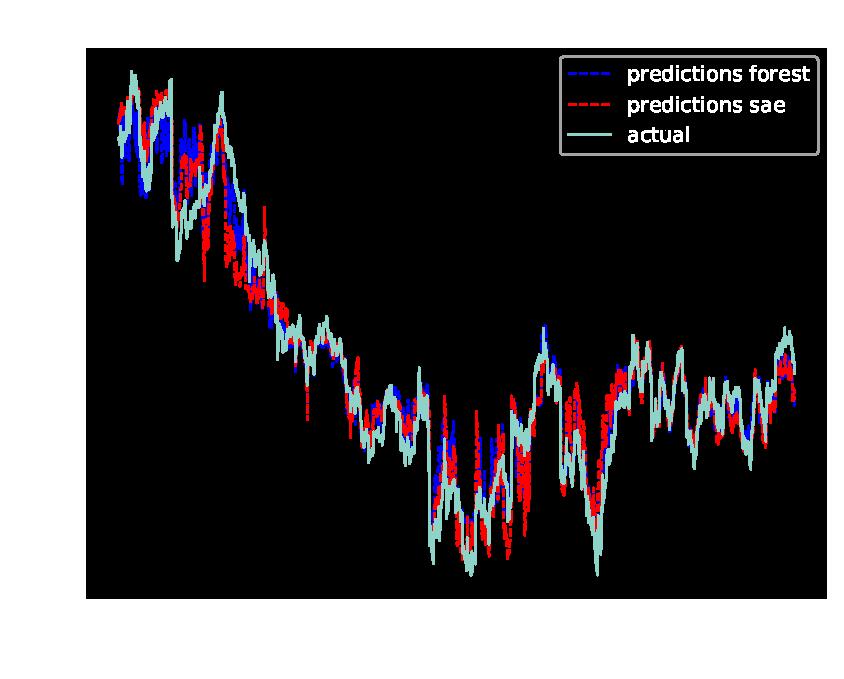
\includegraphics[scale=1]{Appendix3/Figs/rn0f5/NVID_randomSeed_0_forest_no_5_YEAR_2011.png}
%     \qquad
%     \begin{tabular}[b]{|c|c|c|}\hline
%       Field & Forest Encoders & SAE \\ \hline
%       Data & NVidia 2011 & NVidia 2011 \\ \hline
%       Profitability & 65.41\% &18.53\% \\ \hline
%     \end{tabular}
%     \captionlistentry[table]{Results NVidia 2011}
%     \captionsetup{labelformat=andtable}
%     \caption{Comparison of SAE and Forest performances on NVidia 2011 data}
% \end{figure}
% \newpage
% \begin{figure}[!htb]
%     \centering
%     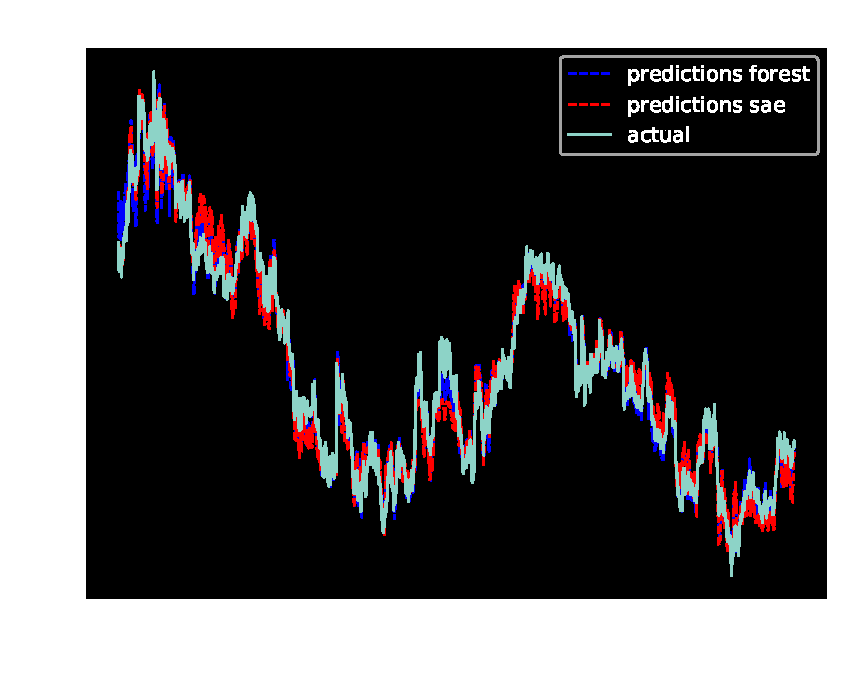
\includegraphics[scale=1]{Appendix3/Figs/rn0f5/NVID_randomSeed_0_forest_no_5_YEAR_2012.png}
%     \qquad
%     \begin{tabular}[b]{|c|c|c|}\hline
%       Field & Forest Encoders & SAE \\ \hline
%       Data & NVidia 2012 & NVidia 2012 \\ \hline
%       Profitability & 42.73\% &36.97\% \\ \hline
%     \end{tabular}
%     \captionlistentry[table]{Results NVidia 2012}
%     \captionsetup{labelformat=andtable}
%     \caption{Comparison of SAE and Forest performances on NVidia 2012 data}
% \end{figure}
% \newpage
% \begin{figure}[!htb]
%     \centering
%     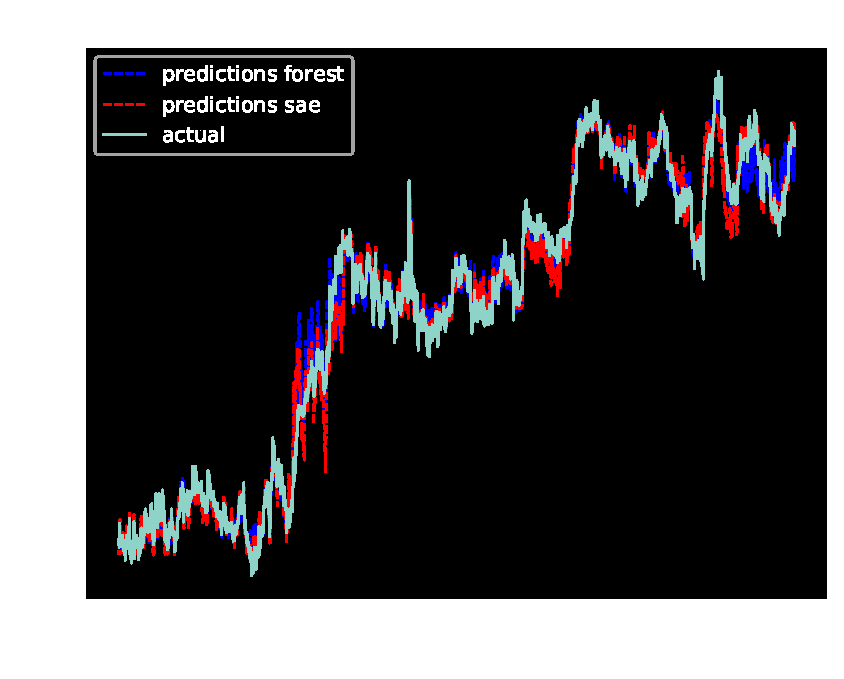
\includegraphics[scale=1]{Appendix3/Figs/rn0f5/NVID_randomSeed_0_forest_no_5_YEAR_2013.png}
%     \qquad
%     \begin{tabular}[b]{|c|c|c|}\hline
%       Field & Forest Encoders & SAE \\ \hline
%       Data & NVidia 2013 & NVidia 2013 \\ \hline
%       Profitability & -9.10\% &-11.98\% \\ \hline
%     \end{tabular}
%     \captionlistentry[table]{Results NVidia 2013}
%     \captionsetup{labelformat=andtable}
%     \caption{Comparison of SAE and Forest performances on NVidia 2013 data}
% \end{figure}
% \newpage
% \begin{figure}[!htb]
%     \centering
%     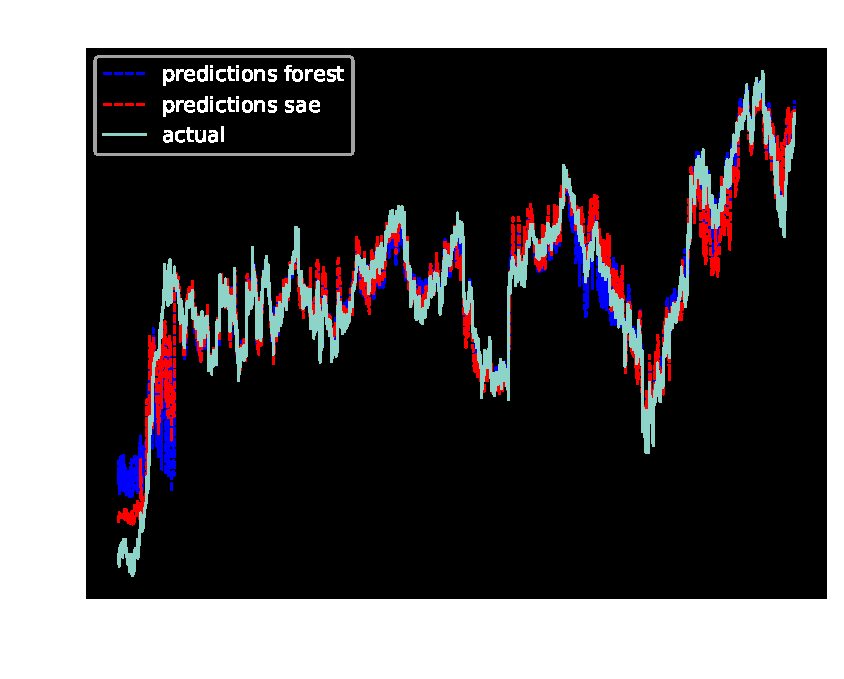
\includegraphics[scale=1]{Appendix3/Figs/rn0f5/NVID_randomSeed_0_forest_no_5_YEAR_2014.png}
%     \qquad
%     \begin{tabular}[b]{|c|c|c|}\hline
%       Field & Forest Encoders & SAE \\ \hline
%       Data & NVidia 2014 & NVidia 2014 \\ \hline
%       Profitability & -17.94\% &-34.30\% \\ \hline
%     \end{tabular}
%     \captionlistentry[table]{Results NVidia 2014}
%     \captionsetup{labelformat=andtable}
%     \caption{Comparison of SAE and Forest performances on NVidia 2014 data}
% \end{figure}
% \newpage
% \begin{figure}[!htb]
%     \centering
%     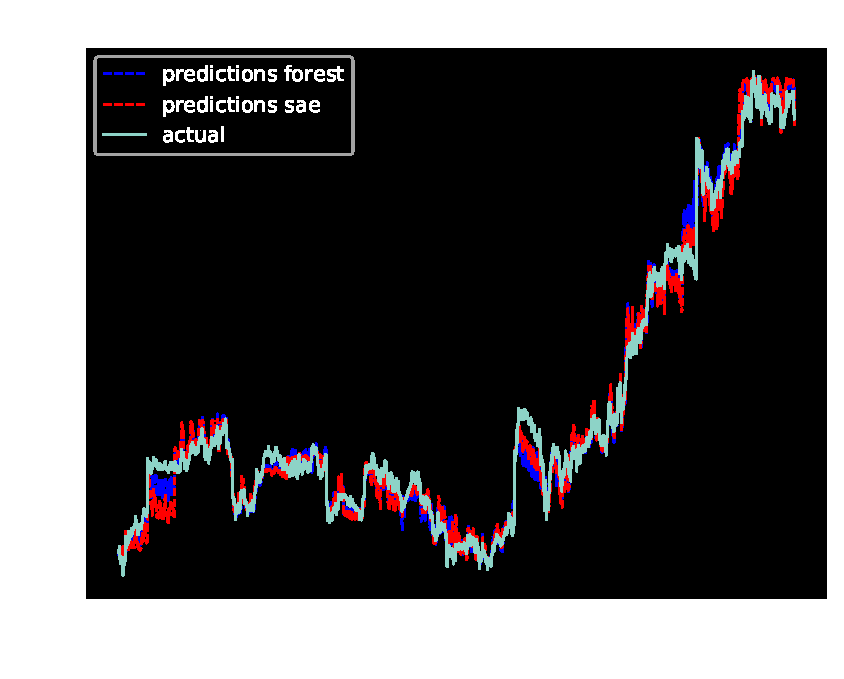
\includegraphics[scale=1]{Appendix3/Figs/rn0f5/NVID_randomSeed_0_forest_no_5_YEAR_2015.png}
%     \qquad
%     \begin{tabular}[b]{|c|c|c|}\hline
%       Field & Forest Encoders & SAE \\ \hline
%       Data & NVidia 2015 & NVidia 2015 \\ \hline
%       Profitability & 13.43\% &-14.32\% \\ \hline
%     \end{tabular}
%     \captionlistentry[table]{Results NVidia 2015}
%     \captionsetup{labelformat=andtable}
%     \caption{Comparison of SAE and Forest performances on NVidia 2015 data}
% \end{figure}
% \newpage
% \begin{figure}[!htb]
%     \centering
%     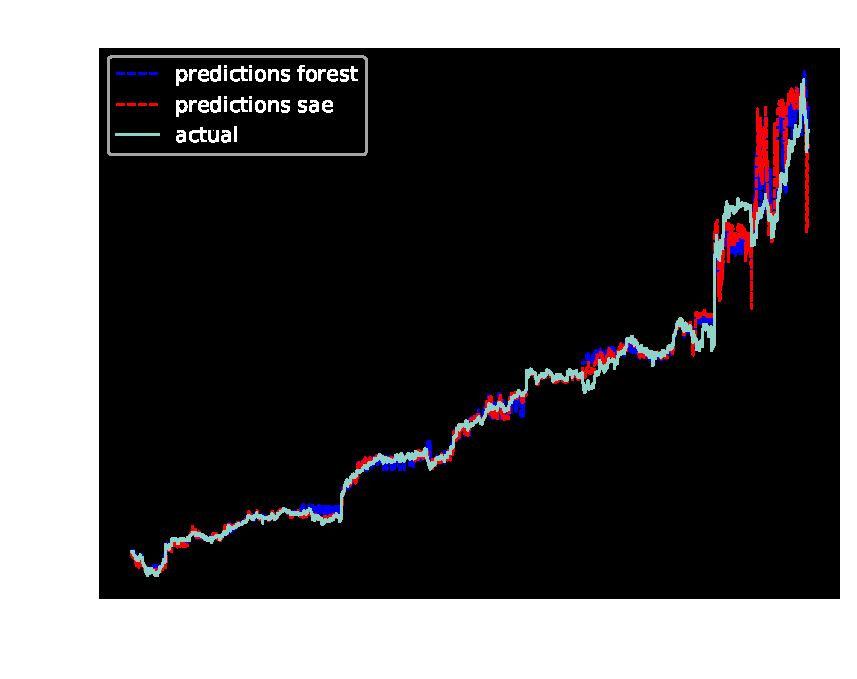
\includegraphics[scale=1]{Appendix3/Figs/rn0f5/NVID_randomSeed_0_forest_no_5_YEAR_2016.png}
%     \qquad
%     \begin{tabular}[b]{|c|c|c|}\hline
%       Field & Forest Encoders & SAE \\ \hline
%       Data & NVidia 2016 & NVidia 2016 \\ \hline
%       Profitability & 30.09\% &-17.53\% \\ \hline
%     \end{tabular}
%     \captionlistentry[table]{Results NVidia 2016}
%     \captionsetup{labelformat=andtable}
%     \caption{Comparison of SAE and Forest performances on NVidia 2016 data}
% \end{figure}
% \newpage
% \begin{figure}[!htb]
%     \centering
%     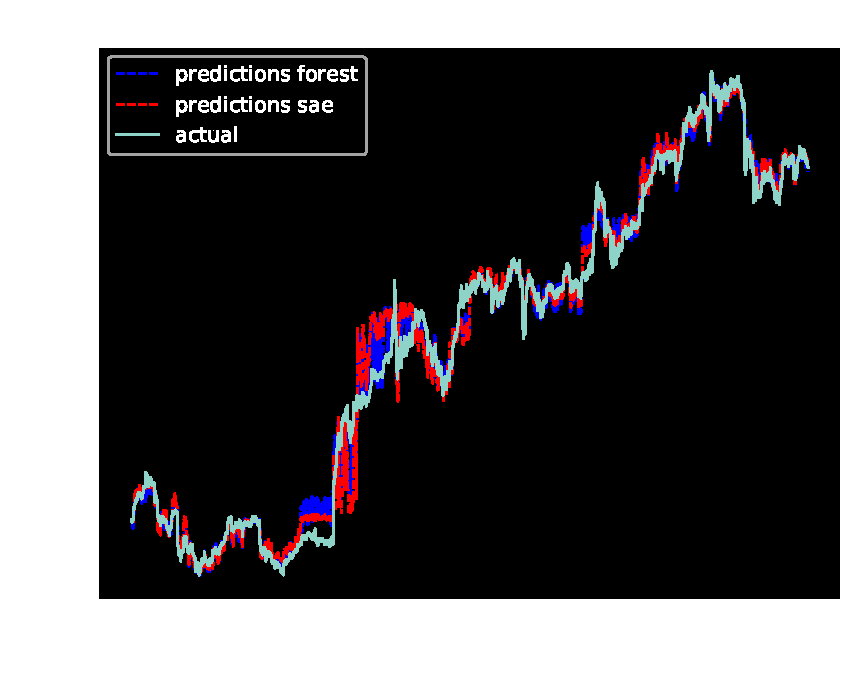
\includegraphics[scale=1]{Appendix3/Figs/rn0f5/NVID_randomSeed_0_forest_no_5_YEAR_2017.png}
%     \qquad
%     \begin{tabular}[b]{|c|c|c|}\hline
%       Field & Forest Encoders & SAE \\ \hline
%       Data & NVidia 2017 & NVidia 2017 \\ \hline
%       Profitability & 45.69\% &-8.91\% \\ \hline
%     \end{tabular}
%     \captionlistentry[table]{Results NVidia 2017}
%     \captionsetup{labelformat=andtable}
%     \caption{Comparison of SAE and Forest performances on NVidia 2017 data}
% \end{figure}
% \newpage

% \subsection*{Philip Morris Overall results}
% \begin{tabular}[!htb]{|c|c|c|}\hline
%       Field & Forest Encoders & SAE \\ \hline
%       Features encoded & 5 & 7 \\ \hline
%       Total Time(6 years) (seconds) & 895.51 & 975.85 \\ \hline
%       Encoding Time (seconds) & 0.34 & 26.44 \\ \hline
%       Total Profitability & 10.61\% & -39.18\% \\ \hline
%       Average Profitability & 1.17\% & -4.35\% \\ \hline
% \end{tabular}
% \newpage
% \subsection*{Philip Morris Yearly results}

% \begin{figure}[!htb]
%     \centering
%     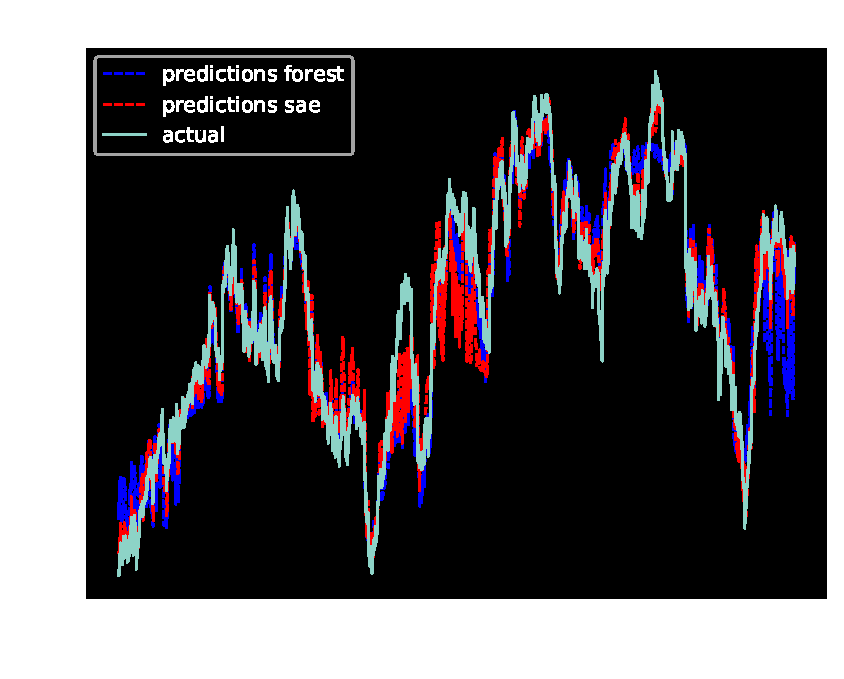
\includegraphics[scale=1]{Appendix3/Figs/rn0f5/PM-1_randomSeed_0_forest_no_5_YEAR_2012.png}
%     \qquad
%     \begin{tabular}[b]{|c|c|c|}\hline
%       Field & Forest Encoders & SAE \\ \hline
%       Data & Philip Morris 2012 & Philip Morris 2012 \\ \hline
%       Profitability & 5.88\% &-9.82\% \\ \hline
%     \end{tabular}
%     \captionlistentry[table]{Results Philip Morris 2012}
%     \captionsetup{labelformat=andtable}
%     \caption{Comparison of SAE and Forest performances on Philip Morris 2012 data}
% \end{figure}
% \newpage
% \begin{figure}[!htb]
%     \centering
%     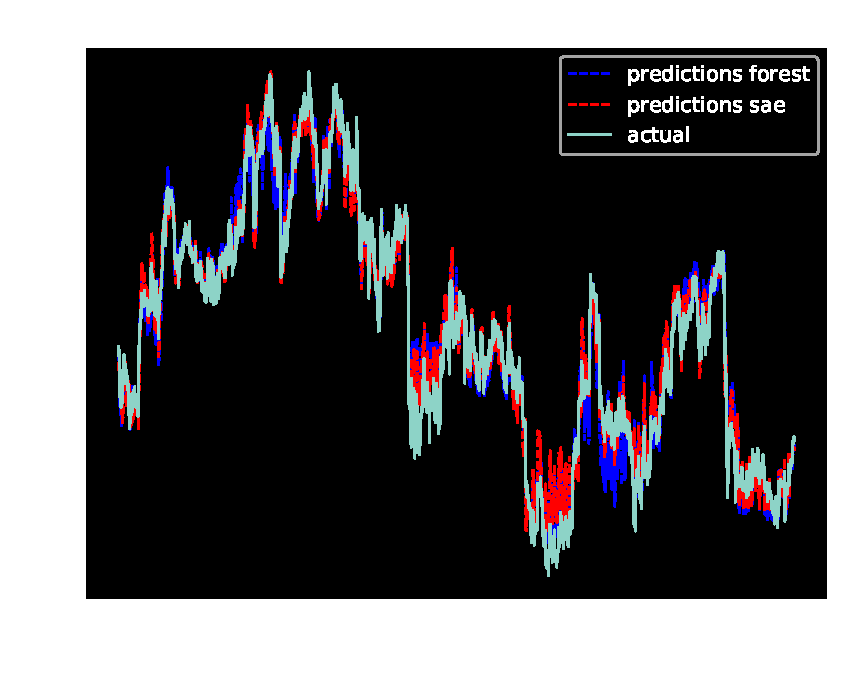
\includegraphics[scale=1]{Appendix3/Figs/rn0f5/PM-1_randomSeed_0_forest_no_5_YEAR_2013.png}
%     \qquad
%     \begin{tabular}[b]{|c|c|c|}\hline
%       Field & Forest Encoders & SAE \\ \hline
%       Data & Philip Morris 2013 & Philip Morris 2013 \\ \hline
%       Profitability & 15.51\% &1.67\% \\ \hline
%     \end{tabular}
%     \captionlistentry[table]{Results Philip Morris 2013}
%     \captionsetup{labelformat=andtable}
%     \caption{Comparison of SAE and Forest performances on Philip Morris 2013 data}
% \end{figure}
% \newpage
% \begin{figure}[!htb]
%     \centering
%     \includegraphics[scale=1]{Appendix3/Figs/rn0f5/PM-1_randomSeed_0_forest_no_5_YEAR_2014.png}
%     \qquad
%     \begin{tabular}[b]{|c|c|c|}\hline
%       Field & Forest Encoders & SAE \\ \hline
%       Data & Philip Morris 2014 & Philip Morris 2014 \\ \hline
%       Profitability & -1.42\% &7.37\% \\ \hline
%     \end{tabular}
%     \captionlistentry[table]{Results Philip Morris 2014}
%     \captionsetup{labelformat=andtable}
%     \caption{Comparison of SAE and Forest performances on Philip Morris 2014 data}
% \end{figure}
% \newpage
% \begin{figure}[!htb]
%     \centering
%     \includegraphics[scale=1]{Appendix3/Figs/rn0f5/PM-1_randomSeed_0_forest_no_5_YEAR_2015.png}
%     \qquad
%     \begin{tabular}[b]{|c|c|c|}\hline
%       Field & Forest Encoders & SAE \\ \hline
%       Data & Philip Morris 2015 & Philip Morris 2015 \\ \hline
%       Profitability & 11.20\% &22.79\% \\ \hline
%     \end{tabular}
%     \captionlistentry[table]{Results Philip Morris 2015}
%     \captionsetup{labelformat=andtable}
%     \caption{Comparison of SAE and Forest performances on Philip Morris 2015 data}
% \end{figure}
% \newpage
% \begin{figure}[!htb]
%     \centering
%     \includegraphics[scale=1]{Appendix3/Figs/rn0f5/PM-1_randomSeed_0_forest_no_5_YEAR_2016.png}
%     \qquad
%     \begin{tabular}[b]{|c|c|c|}\hline
%       Field & Forest Encoders & SAE \\ \hline
%       Data & Philip Morris 2016 & Philip Morris 2016 \\ \hline
%       Profitability & -24.77\% &-40.28\% \\ \hline
%     \end{tabular}
%     \captionlistentry[table]{Results Philip Morris 2016}
%     \captionsetup{labelformat=andtable}
%     \caption{Comparison of SAE and Forest performances on Philip Morris 2016 data}
% \end{figure}
% \newpage
% \begin{figure}[!htb]
%     \centering
%     \includegraphics[scale=1]{Appendix3/Figs/rn0f5/PM-1_randomSeed_0_forest_no_5_YEAR_2017.png}
%     \qquad
%     \begin{tabular}[b]{|c|c|c|}\hline
%       Field & Forest Encoders & SAE \\ \hline
%       Data & Philip Morris 2017 & Philip Morris 2017 \\ \hline
%       Profitability & 4.20\% &-20.92\% \\ \hline
%     \end{tabular}
%     \captionlistentry[table]{Results Philip Morris 2017}
%     \captionsetup{labelformat=andtable}
%     \caption{Comparison of SAE and Forest performances on Philip Morris 2017 data}
% \end{figure}
% \newpage

% \subsection*{Ralph Lauren Overall results}
% \begin{tabular}[!htb]{|c|c|c|}\hline
%       Field & Forest Encoders & SAE \\ \hline
%       Features encoded & 5 & 7 \\ \hline
%       Total Time(6 years) (seconds) & 932.75 & 995.04 \\ \hline
%       Encoding Time (seconds) & 0.35 & 26.95 \\ \hline
%       Total Profitability & 34.59\% & -33.85\% \\ \hline
%       Average Profitability & 3.84\% & -3.76\% \\ \hline
% \end{tabular}
% \newpage
% \subsection*{Philip Morris Yearly results}

% \begin{figure}[!htb]
%     \centering
%     \includegraphics[scale=1]{Appendix3/Figs/rn0f5/RL_1_randomSeed_0_forest_no_5_YEAR_2012.png}
%     \qquad
%     \begin{tabular}[b]{|c|c|c|}\hline
%       Field & Forest Encoders & SAE \\ \hline
%       Data & Ralph Lauren 2012 & Ralph Lauren 2012 \\ \hline
%       Profitability & 16.85\% &24.85\% \\ \hline
%     \end{tabular}
%     \captionlistentry[table]{Results Ralph Lauren 2012}
%     \captionsetup{labelformat=andtable}
%     \caption{Comparison of SAE and Forest performances on Ralph Lauren 2012 data}
% \end{figure}
% \newpage
% \begin{figure}[!htb]
%     \centering
%     \includegraphics[scale=1]{Appendix3/Figs/rn0f5/RL_1_randomSeed_0_forest_no_5_YEAR_2013.png}
%     \qquad
%     \begin{tabular}[b]{|c|c|c|}\hline
%       Field & Forest Encoders & SAE \\ \hline
%       Data & Ralph Lauren 2013 & Ralph Lauren 2013 \\ \hline
%       Profitability & -3.57\% &-2.18\% \\ \hline
%     \end{tabular}
%     \captionlistentry[table]{Results Ralph Lauren 2013}
%     \captionsetup{labelformat=andtable}
%     \caption{Comparison of SAE and Forest performances on Ralph Lauren 2013 data}
% \end{figure}
% \newpage
% \begin{figure}[!htb]
%     \centering
%     \includegraphics[scale=1]{Appendix3/Figs/rn0f5/RL_1_randomSeed_0_forest_no_5_YEAR_2014.png}
%     \qquad
%     \begin{tabular}[b]{|c|c|c|}\hline
%       Field & Forest Encoders & SAE \\ \hline
%       Data & Ralph Lauren 2014 & Ralph Lauren 2014 \\ \hline
%       Profitability & 6.67\% &38.49\% \\ \hline
%     \end{tabular}
%     \captionlistentry[table]{Results Ralph Lauren 2014}
%     \captionsetup{labelformat=andtable}
%     \caption{Comparison of SAE and Forest performances on Ralph Lauren 2014 data}
% \end{figure}
% \newpage
% \begin{figure}[!htb]
%     \centering
%     \includegraphics[scale=1]{Appendix3/Figs/rn0f5/RL_1_randomSeed_0_forest_no_5_YEAR_2015.png}
%     \qquad
%     \begin{tabular}[b]{|c|c|c|}\hline
%       Field & Forest Encoders & SAE \\ \hline
%       Data & Ralph Lauren 2015 & Ralph Lauren 2015 \\ \hline
%       Profitability & 24.11\% &-17.69\% \\ \hline
%     \end{tabular}
%     \captionlistentry[table]{Results Ralph Lauren 2015}
%     \captionsetup{labelformat=andtable}
%     \caption{Comparison of SAE and Forest performances on Ralph Lauren 2015 data}
% \end{figure}
% \newpage
% \begin{figure}[!htb]
%     \centering
%     \includegraphics[scale=1]{Appendix3/Figs/rn0f5/RL_1_randomSeed_0_forest_no_5_YEAR_2016.png}
%     \qquad
%     \begin{tabular}[b]{|c|c|c|}\hline
%       Field & Forest Encoders & SAE \\ \hline
%       Data & Ralph Lauren 2016 & Ralph Lauren 2016 \\ \hline
%       Profitability & -13.29\% &-57.98\% \\ \hline
%     \end{tabular}
%     \captionlistentry[table]{Results Ralph Lauren 2016}
%     \captionsetup{labelformat=andtable}
%     \caption{Comparison of SAE and Forest performances on Ralph Lauren 2016 data}
% \end{figure}
% \newpage
% \begin{figure}[!htb]
%     \centering
%     \includegraphics[scale=1]{Appendix3/Figs/rn0f5/RL_1_randomSeed_0_forest_no_5_YEAR_2017.png}
%     \qquad
%     \begin{tabular}[b]{|c|c|c|}\hline
%       Field & Forest Encoders & SAE \\ \hline
%       Data & Ralph Lauren 2017 & Ralph Lauren 2017 \\ \hline
%       Profitability & 3.80\% &-19.35\% \\ \hline
%     \end{tabular}
%     \captionlistentry[table]{Results Ralph Lauren 2017}
%     \captionsetup{labelformat=andtable}
%     \caption{Comparison of SAE and Forest performances on Ralph Lauren 2017 data}
% \end{figure}
% \newpage